
%***************************************************************************
%
% CreditCruncher - A portfolio credit risk valorator
% Copyright (C) 2004 Gerard Torrent
%
% This program is free software; you can redistribute it and/or
% modify it under the terms of the GNU General Public License
% as published by the Free Software Foundation; either version 2
% of the License.
%
% This program is distributed in the hope that it will be useful,
% but WITHOUT ANY WARRANTY; without even the implied warranty of
% MERCHANTABILITY or FITNESS FOR A PARTICULAR PURPOSE.  See the
% GNU General Public License for more details.
%
% You should have received a copy of the GNU General Public License
% along with this program; if not, write to the Free Software
% Foundation, Inc., 59 Temple Place - Suite 330, Boston, MA 02111-1307, USA.
%
%
% user.tex - TeX documentation file
% --------------------------------------------------------------------------
%
% 2004/12/04 - Gerard Torrent [gerard@fobos.generacio.com]
%   . initial release
% 
% 2005/04/13 - Gerard Torrent [gerard@fobos.generacio.com]
%   . some format enhancements
%
%***************************************************************************

\documentclass[a4paper,11pt,final]{report}
%\usepackage{times}
\usepackage{latexsym}
\usepackage[dvips]{graphicx}
\usepackage[spanish]{babel}
%\usepackage{fullpage}
\usepackage[final]{listings}
\usepackage{fancyhdr}
\usepackage{eurosym}
\usepackage{makeidx}

%-----------------------------------------------------
% defining some useful values
%-----------------------------------------------------
\def\numversion{0.6}
\def\svnversion{R262M}

%-----------------------------------------------------
% european spacing correction 
%-----------------------------------------------------
\frenchspacing
\sloppy

%-----------------------------------------------------
% set fancy header (see lshort.pdf)
%-----------------------------------------------------
%\pagestyle{headings}
\pagestyle{fancy}
\renewcommand{\chaptermark}[1]{\markboth{#1}{}}
\renewcommand{\sectionmark}[1]{\markright{\thesection\ #1}}
\fancyhf{}
\fancyhead[LE,RO]{\bfseries\thepage}
\fancyhead[LO]{\bfseries\rightmark}
\fancyhead[RE]{\bfseries\leftmark}
\renewcommand{\headrulewidth}{0.5pt}
\renewcommand{\footrulewidth}{0pt}
\addtolength{\headheight}{2.5pt}
\fancypagestyle{plain}{
  \fancyhead{}
  \renewcommand{\headrulewidth}{0pt}
}

%-----------------------------------------------------
% removes initial indentation from paragraphs
%-----------------------------------------------------
\setlength\parindent{0ex}

%-----------------------------------------------------
% enable indexing commands
%-----------------------------------------------------
\makeindex

%-----------------------------------------------------
% finally, the doc begins here
%-----------------------------------------------------
\begin{document}


%***************************************************************************
%
% CreditCruncher - A portfolio credit risk valorator
% Copyright (C) 2004 Gerard Torrent
%
% This program is free software; you can redistribute it and/or
% modify it under the terms of the GNU General Public License
% as published by the Free Software Foundation; either version 2
% of the License.
%
% This program is distributed in the hope that it will be useful,
% but WITHOUT ANY WARRANTY; without even the implied warranty of
% MERCHANTABILITY or FITNESS FOR A PARTICULAR PURPOSE.  See the
% GNU General Public License for more details.
%
% You should have received a copy of the GNU General Public License
% along with this program; if not, write to the Free Software
% Foundation, Inc., 59 Temple Place - Suite 330, Boston, MA 02111-1307, USA.
%
%
% titlepage.tex - TeX documentation file
% --------------------------------------------------------------------------
%
% 2004/12/04 - Gerard Torrent [gerard@fobos.generacio.com]
%   . initial release
%
%***************************************************************************

\title{CreditCruncher - Technical Document \\
Version 0.5 \\
\ \\
\centerline{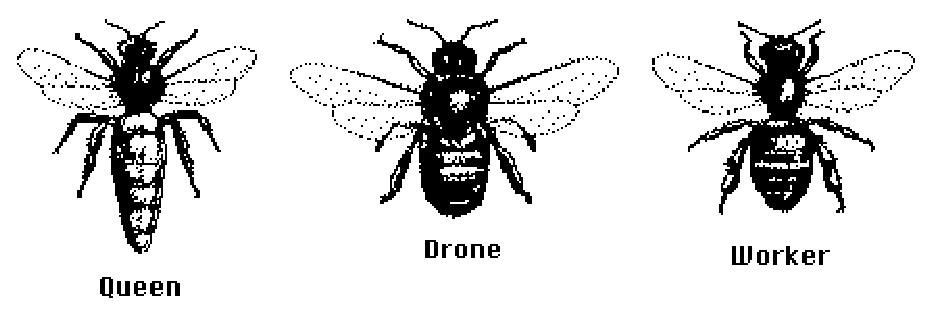
\includegraphics[height=3cm, angle=0]{./images/threebees.eps}}
}

\author{Gerard Torrent Gironella}

\maketitle

\thispagestyle{empty}

\newpage

\vspace*{6in}

\noindent Copyright $\copyright$ 2004-2005 Gerard Torrent Gironella.\\

\noindent The image found in cover have been taken from Mark L. Winston. 1987. 
\emph{The Biology of the Honey Bee} (ISBN: 0-671-07109-2). Harvard University 
Press. Cambridge, MA. These redrawn figures appear here without permission of 
Harvard University Press [Ref: 973029].\\

\noindent This file is part of the CreditCruncher software package.  For
license information, see the COPYING file in the top level directory
of the CreditCruncher source distribution.

\tableofcontents
%\listoftables


%***************************************************************************
%
% CreditCruncher - A portfolio credit risk valorator
% Copyright (C) 2004 Gerard Torrent
%
% This program is free software; you can redistribute it and/or
% modify it under the terms of the GNU General Public License
% as published by the Free Software Foundation; either version 2
% of the License.
%
% This program is distributed in the hope that it will be useful,
% but WITHOUT ANY WARRANTY; without even the implied warranty of
% MERCHANTABILITY or FITNESS FOR A PARTICULAR PURPOSE.  See the
% GNU General Public License for more details.
%
% You should have received a copy of the GNU General Public License
% along with this program; if not, write to the Free Software
% Foundation, Inc., 59 Temple Place - Suite 330, Boston, MA 02111-1307, USA.
%
%
% introduction.tex - TeX documentation file
% --------------------------------------------------------------------------
%
% 2004/12/04 - Gerard Torrent [gerard@fobos.generacio.com]
%   . initial release
%
%***************************************************************************

\chapter{Introduction to CreditCruncher}
\label{sec:introduction}

\section{About CreditCruncher}

CreditCruncher valora el riesgo de impago de una cartera de cr\'editos usando la 
t\'ecnica de simulaci\'on Monte Carlo. Es una implementaci\'on libre de la metodologia
CreditMetrics\footnote{http://www.riskmetrics.com/}. 

Se dispone de una cartera de N clientes donde cada cliente tiene contratado uno o 
varios productos con riesgo de cr\'edito. Cada cliente tiene asignado un rating de 
calidad crediticia y existe una matriz de transici\'on que permite determinar la 
probabilidad de fallido a un horizonte de tiempo fijado. Los clientes pertenecen 
a diversos sectores de los que disponemos de una matriz de correlaci\'on que 
indica el grado de dependencia intersectorial en caso de fallido. A partir de 
la matriz de correlaci\'on intersectorial se construye la matriz de correlaci\'on 
entre clientes. Finalmente se genera un conjunto de N variables aleatorias 
uniformes correlacionadas seg\'un esta matriz (c\'opula). Se usa la matriz de 
transici\'on para determinar la evoluci\'on del rating inicial de cada cliente y se 
evalua el valor de sus productos. Si se repite este proceso un n\'umero elevado de 
veces disponemos de un conjunto de valores posibles de la cartera que permiten 
determinar la distribuci\'on del valor de la cartera y calcular el VAR (Value At Risk). 
Para mas informaci\'on cons\'ultese el manual de CreditCruncher donde se describe 
con detalle todos los pasos realizados.


\chapter{Formulaci\'on del problema}
\label{sec:formulation}

\section{Hipotesis}

\paragraph{La \'unica fuente de riesgo es el riesgo de impago.}
No se contemplan los riesgos de variaci\'on de tipos de inter\'es, etc.

\paragraph{El tiempo est\'a repartido uniformemente.}
blablabla.

\paragraph{Un fallido no se recupera.}
blablabla.

\paragraph{Las probabilidades de fallido no dependen del tiempo.}
blablabla.

\paragraph{El rating y la recuperaci\'on de un cliente no depende de otro cliente.}
blablabla.


%===========================================================================

\section{La matriz de transici\'on}

\subsection{Definici\'on.} La matriz de transici\'on nos proporciona la probabilidad 
que un cliente con rating inicial $r_i$ pase a tener, al cabo de un tiempo $T$, 
rating $r_j$. La denotamos de la forma siguiente:

\begin{displaymath}
M_T = \left(
\begin{array}{ccc}
m_{1,1} & \dots  & m_{1,n} \cr
\vdots & \ddots & \vdots \cr
m_{n,1} & \dots  & m_{n,n} 
\end{array}
\right)
\end{displaymath}

\noindent donde cada elemento de la matrix, $m_{i,j}$ corresponde a la 
probabilidad de que un cliente con rating $r_i$ pase a tener, al cabo de $T$ 
tiempo, rating $r_j$.

\subsection{Ejemplo.} Matriz de transici\'on anual ($T=1$ año) extraida del 
documento \emph{CreditMetrics. Technical Document}. Las probabilidades est\'an
expresadas en tanto por ciento.
\\
\begin{center}
\begin{tabular}[]{l|rrrrrrrr}
        &      AAA &       AA &        A &      BBB &       BB &        B &      CCC &  Default \cr
\hline
AAA     &  $90.81$ &   $8.33$ &   $0.68$ &   $0.06$ &   $0.12$ &   $0.00$ &   $0.00$ &   $0.00$ \cr
 AA     &   $0.70$ &  $90.65$ &   $7.79$ &   $0.64$ &   $0.06$ &   $0.14$ &   $0.02$ &   $0.00$ \cr
  A     &   $0.09$ &   $2.27$ &  $91.05$ &   $5.52$ &   $0.74$ &   $0.26$ &   $0.01$ &   $0.06$ \cr
BBB     &   $0.02$ &   $0.33$ &   $5.95$ &  $86.93$ &   $5.30$ &   $1.17$ &   $0.12$ &   $0.18$ \cr
 BB     &   $0.03$ &   $0.14$ &   $0.67$ &   $7.73$ &  $80.53$ &   $8.84$ &   $1.00$ &   $1.06$ \cr
  B     &   $0.00$ &   $0.11$ &   $0.24$ &   $0.43$ &   $6.48$ &  $83.46$ &   $4.07$ &   $5.20$ \cr
CCC     &   $0.22$ &   $0.00$ &   $0.22$ &   $1.30$ &   $2.38$ &  $11.24$ &  $64.86$ &  $19.79$ \cr
Default &   $0.00$ &   $0.00$ &   $0.00$ &   $0.00$ &   $0.00$ &   $0.00$ &   $0.00$ & $100.00$
\end{tabular}
\end{center}
\noindent en particular, la probabilidad que un cliente con rating $AA$ pase a 
tener rating $B$ al cabo de un año es del $0.14\%$.

\subsection{Propiedades}

\paragraph{Propiedad 1.}
El valor de los elementos de la matriz de transici\'on se encuentran entre $0$ 
y $1$ debido a que son probabilidades.

\begin{displaymath}
0 \leq m_{i,j} \leq 1 \quad \forall i,j
\end{displaymath}

\paragraph{Propiedad 2.}
La suma de los elementos de cualquier fila de la matriz de transici\'on suman $1$.
De esta forma se  est\'a imponiendo que el conjunto de ratings finales solo puede 
ser el de los ratings contemplados en la matriz.

\begin{displaymath}
\sum_{j=1}^{n} m_{i,j} = 1 \quad \forall i
\end{displaymath}

\paragraph{Propiedad 3.}
Los elementos de la fila correspondiente al rating $default$, son todos $0$,
excepto el elemento de la columna que corresponde al rating $default$ que vale 
$1$. Esta condici\'on indica que cuando se llega al estado de fallido no es 
posible salir de este estado.

\begin{displaymath}
\begin{array}{ll}
m_{default,j} = 0        & \quad \forall j \neq default \cr
m_{default,default} = 1
\end{array}
\end{displaymath}


\subsection{Cambio de periodo}

Deseamos obtener la matriz de transici\'on para periodos distintos (m\'ultiplos o 
fraccionarios) del periodo proporcionado, $T$. Esto nos permitir\'a determinar la 
probabilidad que un cliente con rating inicial $r_i$ tenga rating $r_j$ al cabo 
de $x \cdot T$ tiempo.

\paragraph{Ejemplo.} Calculemos la probabilidad de pasar de rating $AA$ a
rating $B$ en un plazo de dos años disponiendo de la matriz de transici\'on anual.

\begin{displaymath}
\begin{array}{llll}
P(AA \to B;2) = & P(AA \to AAA;1)    & \cdot P(AAA \to B;1)      & + \cr
                & P(AA \to AA;1)      & \cdot P(AA \to B;1)      & + \cr
                & P(AA \to A;1)       & \cdot P(A \to B;1)       & + \cr
                & P(AA \to BBB;1)     & \cdot P(BBB \to B;1)     & + \cr
                & P(AA \to BB;1)      & \cdot P(BB \to B;1)      & + \cr
                & P(AA \to B;1)       & \cdot P(B \to B;1)       & + \cr
                & P(AA \to CCC;1)     & \cdot P(CCC \to B;1)     & + \cr
                & P(AA \to default;1) & \cdot P(default \to B;1) &
\end{array}
\end{displaymath}

\paragraph{Proposici\'on} Sean $M_{T_1}$ y $M_{T_2}$ las matrices de transici\'on
para los periodos $T_1$ y $T_2$. Entonces, la matriz de transici\'on para el
periodo $T_1+T_2$ es:
\begin{displaymath}
M_{T_1+T_2} = M_{T_1} \cdot M_{T_2}
\end{displaymath}

\paragraph{Corolario} Sean $M_{T}$ la matriz de transici\'on para el periodo 
$T$ y $k \in \mathrm{N}$. Entonces:
\begin{displaymath}
M_{k \cdot T} = M_{T}^k
\end{displaymath}
\begin{displaymath}
M_{\frac{T}{k}} = \sqrt[k]{M_{T}}
\end{displaymath}


%===========================================================================

\section{C\'alculo de la raiz de una matriz}

\paragraph{Definici\'on.}
Diremos que 2 matrices $A$ y $B$ de orden $n$ son semejantes si existe una 
matriz, $P$, de orden $n$ con $det(P) \neq 0$ tal que 
$B = P^{-1} \cdot A \cdot P$.


\paragraph{Proposici\'on.} Si dos matrices $A$ y $B$ son semejantes 
($B = P^{-1} \cdot A \cdot P$) entonces:
\begin{displaymath}
det(A) = det(B)
\end{displaymath}
\begin{displaymath}
B^n = P^{-1} \cdot A^{n} \cdot P
\end{displaymath}

\paragraph{Definici\'on.} 
Diremos que Una matriz $A$ de orden $n$ es diagonalizable si es semejante a una 
matriz diagonal $D$, o sea, $A = P^{-1} \cdot D \cdot P$ siendo $det(D) \neq 0$.

\paragraph{Proposici\'on.} 
Para que una matriz $A$ sea diagonalizable es necesario y suficiente que:
\begin{itemize}
\item Los valores propios de $A$ sean todos reales
\item Los $n$ vectores propios de $A$ sean independientes
\end{itemize}

\paragraph{Proposici\'on.}
Si una matriz $A$ es diagonalizable ($A = P^{-1} \cdot D \cdot P$) entonces: 
\begin{itemize}
\item $D$ es una matriz diagonal compuesta por los valores propios de la matriz $A$
\item $P$ es la matriz formada por los vectores propios de la matriz $A$
\end{itemize}

\paragraph{Resultado.}
Sea $A$ la ra\'iz $n$-esima de una matriz diagonalizable $B$. Entonces:
\begin{displaymath}
A^n = B = P^{-1} \cdot D \cdot P 
\Longrightarrow  
A = \sqrt[n]{B} = P^{-1} \cdot \sqrt[n]{D} \cdot P
\end{displaymath} 


%===========================================================================

\section{La variable aleatoria normal}

\subsection{Definici\'on y propiedades}

\begin{displaymath}
P(X \leq x) = \Phi(x) = \int_{-\infty}^{x} \frac{e^{-t^2}}{\sqrt{2 \pi}} dt
\end{displaymath}

\subsection{Simulaci\'on}

Para la generaci\'on de una realizaci\'on, $z$, de una variable aleatoria normal  
$Z \sim N(\mu, \sigma)$ utilizamos el siguiente algoritmo:

\begin{displaymath}
z = \mu + \sigma\cdot \sqrt{-2 \cdot ln(u[0,1])} \cdot cos(2 \cdot \pi \cdot u[0,1])
\end{displaymath}

\noindent donde $u[0,1]$ son realizaciones de una variable aleatoria uniforme 
en el intervalo $[0,1]$.

%===========================================================================

\section{Copulas. Variables aleatorias correlacionadas}

\paragraph{Definici\'on.}
Una copula es la funci\'on de distribuci\'on de un vector aleatorio sobre 
$\Re^n$ donde las funciones de distribuci\'on marginales son $U[0,1]$. 
\begin{displaymath}
C(u_1, \cdots, u_n) = P\{U_1 \leq u_1, \cdots, U_n \leq u_n\}
\end{displaymath}

\paragraph{Proposici\'on.}
$C$ es una c\'opula $\iff C:[0,1]^n \to [0,1]$ y cumple las siguientes 
propiedades:
\begin{itemize}
\item $C(x_1, \cdots, x_n)$ es creciente en cada componente $x_i$
\item $C(1, \cdots, 1, x_i, 1, \cdots, 1) = x_i \quad \forall i \in \{1, \cdots, n\}, x_i \in [0,1]$
\item $\forall (a_1, \cdots, a_n) \in [0,1]^n$ y $\forall (b_1, \cdots, b_n) \in [0,1]^n$ con
$a_i \leq b_i$ se cumple:
\begin{displaymath}
\sum_{i_1=1}^{2} \cdots \sum_{i_n=1}^{2} (-1)^{i_1+\cdots+x_n} C(x_{1i_1},\cdots,x_{ni_n}) \geq 0
\end{displaymath}
\noindent siendo $x_{j1}=a_j$ y $x_{j2}=b_j$ $\quad \forall j \in \{1, \cdots, n\}$
\end{itemize}

\paragraph{Generaci\'on de c\'opulas normales o arquimedianas.}

Sea $(Z_1,\cdots, Z_n)$ un vector aleatorio con marginales $Z_i \sim N(0,1)$ con
\begin{displaymath}
\Sigma = \left( 
\begin{array}{cccc}
1          & \rho_{12} & \ldots & \rho_{1n} \cr
\rho_{21} & 1          & \ldots & \rho_{2n} \cr
\vdots    & \vdots    & \ddots & \vdots   \cr
\rho_{n1} & \rho_{n2} & \ldots & 1
\end{array}
\right)
\end{displaymath}

\noindent siendo $\rho_{ij} = \rho_{ji}$ el coeficiente de correlaci\'on entre 
$Z_i$ y $Z_j$.

\noindent Calculamos la raiz de $\Sigma$ usando el algoritmo de Cholesky. 
De esta forma obtenemos la matriz triengular inferior
\begin{displaymath}
B = 
\left(
\begin{array}{cccc}
b_{11}   & 0        & \ldots & 0       \cr
b_{21}   & b_{22}   & \ldots & 0       \cr
\vdots  & \vdots  & \ddots & \vdots \cr
b_{n1}   & b_{n2}   & \ldots & b_{nn}
\end{array}
\right)
\end{displaymath}

\noindent que cumple $B \cdot B' = \Sigma$

\noindent Generamos una simulaci\'on del vector aleatorio $Y=(Y_1, \cdots, Y_n)'$ 
donde $Y_k \sim N(0,1)$ son variables aleatorias independientes.

\noindent Calculamos $Z = B \cdot Y$. El vector aleatorio resultante, $Z$ tiene
marginales $Z_k \sim N(0,1)$ y se encuentran correlacionadas seg\'un la matriz 
$\Sigma$.

\noindent Calculamos $X = (X_1, \cdots, X_n)'$ de la forma:
\begin{displaymath}
x_i = \Phi^{-1}(y_i)
\end{displaymath}

\noindent donde $\Phi(x) = \int_{-\infty}^{x} \frac{1}{\sqrt{2 \pi}} e^{-t^2} dt$


%***************************************************************************
%
% CreditCruncher - A portfolio credit risk valorator
% Copyright (C) 2004 Gerard Torrent
%
% This program is free software; you can redistribute it and/or
% modify it under the terms of the GNU General Public License
% as published by the Free Software Foundation; either version 2
% of the License.
%
% This program is distributed in the hope that it will be useful,
% but WITHOUT ANY WARRANTY; without even the implied warranty of
% MERCHANTABILITY or FITNESS FOR A PARTICULAR PURPOSE.  See the
% GNU General Public License for more details.
%
% You should have received a copy of the GNU General Public License
% along with this program; if not, write to the Free Software
% Foundation, Inc., 59 Temple Place - Suite 330, Boston, MA 02111-1307, USA.
%
%
% formulation.tex - TeX documentation file
% --------------------------------------------------------------------------
%
% 2005/01/22 - Gerard Torrent [gerard@fobos.generacio.com]
%   . initial release
%
%***************************************************************************

\chapter{Formulaci\'on del problema}
\label{sec:formulation}

\begin{center}
\framebox{
\begin{minipage}[c]{12.5cm}
Dada una cartera de cr\'editos a empresas de tama\~no mediano, deseamos 
valorar las posibles p\'erdidas debido a los impagos al cabo de un 
tiempo $T$.
\end{minipage}
}
\end{center}

A continuaci\'on se introduce los elementos y propiedades b\'asicas que 
constituyen el marco de trabajo.

%---------------------------------------------------------------------------

\section{Cartera de cr\'editos}

La estructura de la cartera de cr\'editos consiste en un conjunto de
clientes agrupados por sectores de actividad. Cada cliente tiene contratado 
un conjunto de productos de cr\'edito. Cada contrato puede estar 
cubierto por un n\'umero variable de garant\'ias o acuerdos.
Puede verse un esquema de la estructura en la figura \ref{portfolio}.

\begin{figure}[!hb]
\begin{center}
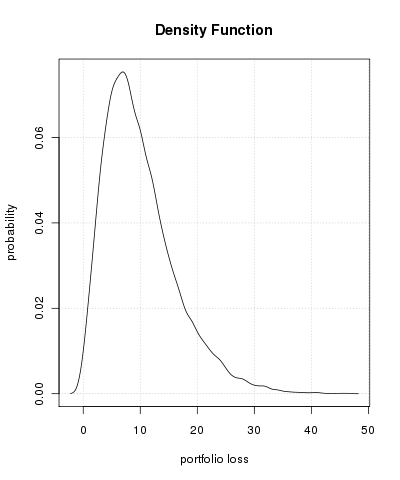
\includegraphics[width=6cm,angle=-90]{./images/portfolio.epsi}
\caption{Estructura de la cartera de cr\'editos}
\label{portfolio}
\end{center}
\end{figure}


\subsection{Ratings}

Un \emph{sistema de ratings}\index{Sistema de ratings} es una medida de calidad
crediticia usada para valorar creditores. A cada creditor se le asigna una nota
discreta (pe. AAA, AA, A, BBB, BB, B, CCC, Default) en funci\'on de su calidad
crediticia. Los \'unicos ratings contemplados en este documento 
son los que tienen una relaci\'on estad\'istica directa y cuantificable 
con la probabilidad de impago del creditor. Ejemplos de este tipo de ratings 
son los publicados por Moody's Investor Service\footnote{http://www.moodys.com} 
o Standard \& Poors\footnote{http://www.standardandpoors.com}. 
\newline
\newline
La metodolog\'ia para la generaci\'on de un sistema de ratings queda fuera del
\'ambito de este documento. CreditCruncher presupone que cada empresa de la 
cartera tiene un rating inicial asignado.
\newline
\newline
El rating de cada empresa puede variar a lo largo del tiempo (v\'ease figura
\ref{ratingevol}). La evoluci\'on temporal del rating de una empresa se
contempla a trav\'es de la matriz de transici\'on o la funci\'on de 
supervivencia (v\'ease la secci\'on \ref{sec:mtransition}).
\begin{figure}[!hb]
\begin{center}
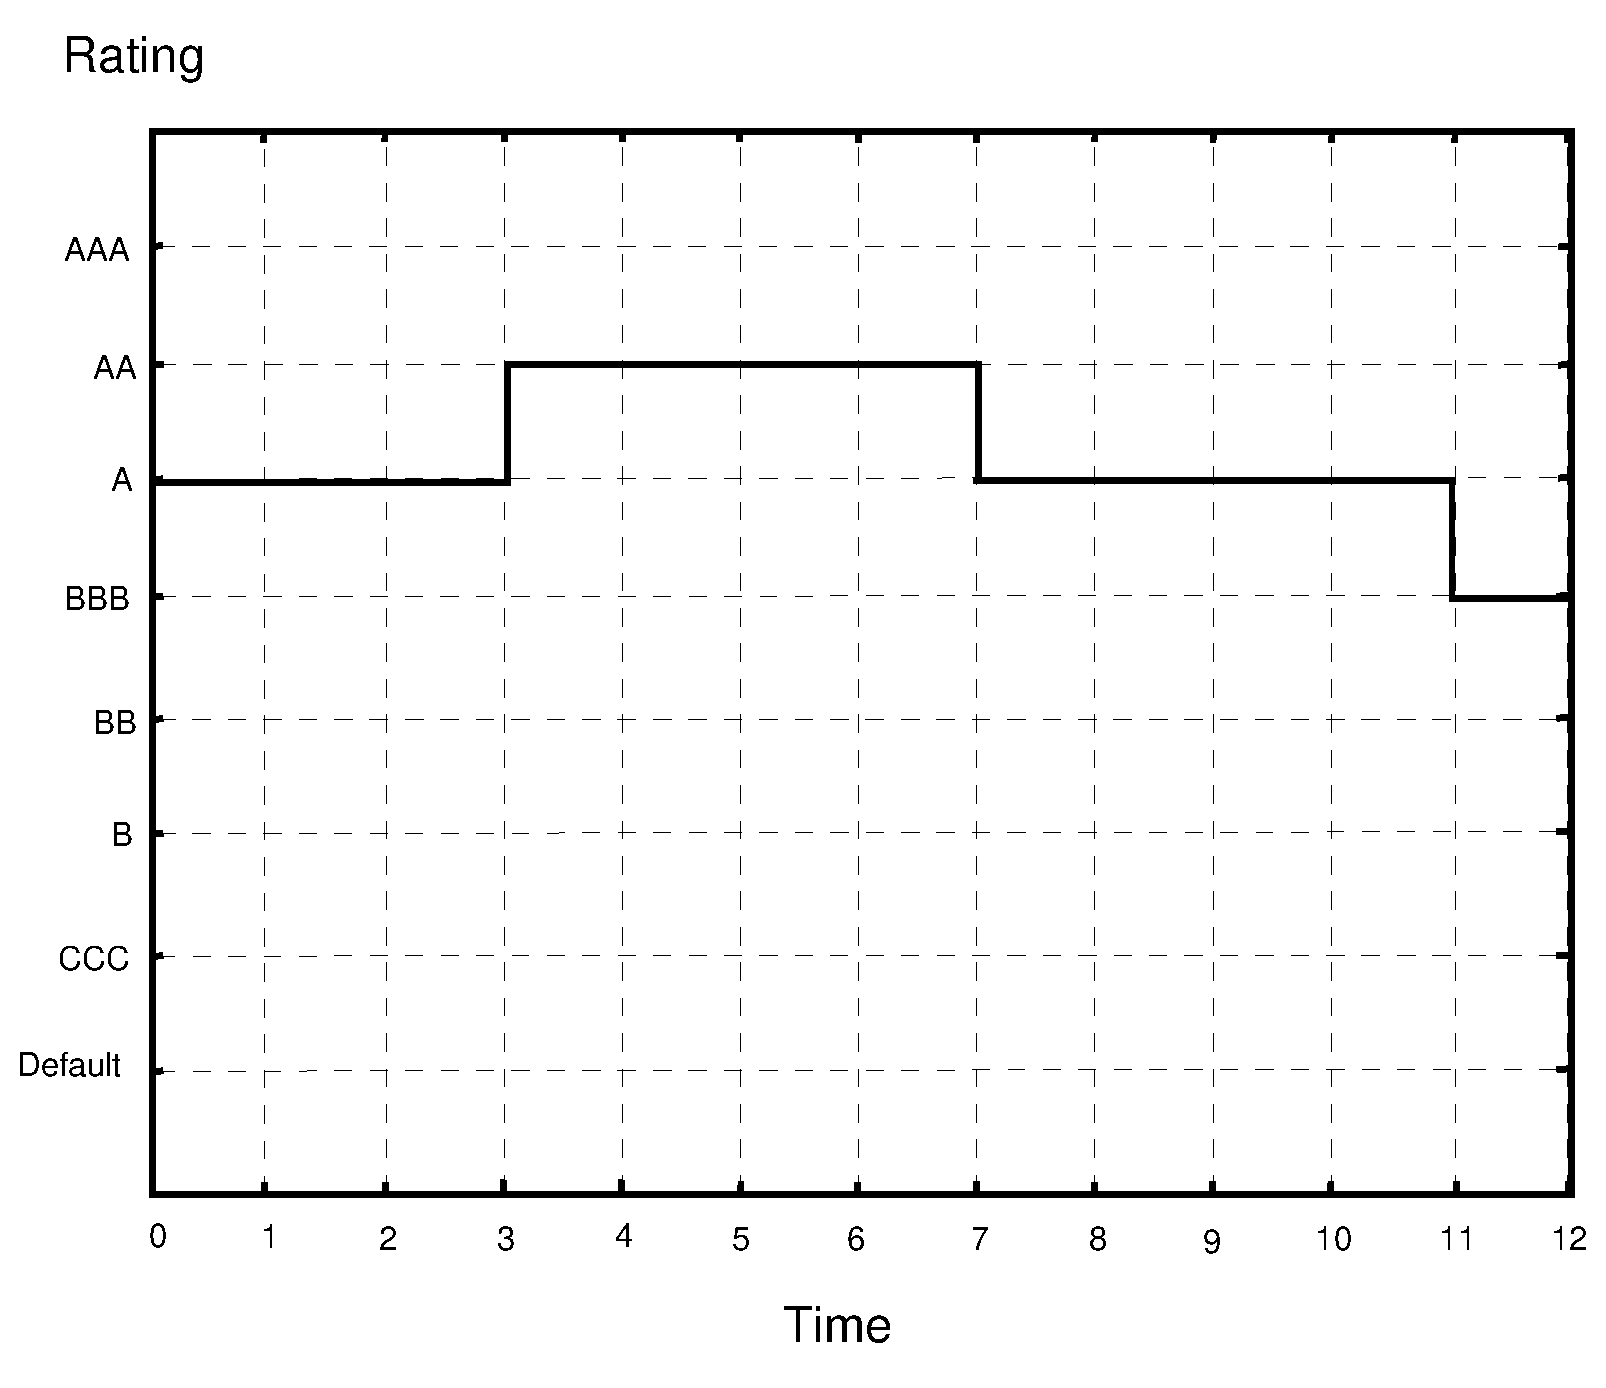
\includegraphics[height=6cm, angle=0]{./images/ratingevol.eps}
\caption{Evoluci\'on del rating a lo largo del tiempo}
\label{ratingevol}
\end{center}
\end{figure}

\paragraph{Notaci\'on.} $P(r_i \to r_j;t_0;t_1) =$ probabilidad de pasar de un 
rating inicial $r_i$ en tiempo $t_0$ a un rating $r_j$ en tiempo $t_1$.


\subsection{Sectores}

La correlaci\'on de fallidos entre clientes es uno de los conceptos que
a\~naden complejidad de la valoraci\'on del riesgo de cr\'edito. No es lo
mismo tener una cartera de cr\'editos donde los clientes hacen fallido 
de forma independiente que una cartera donde los fallidos se encuentran 
correlacionados. En el primer caso, al cabo de un a\~no tendremos un 
conjunto limitado de fallidos. En el segundo caso, al cabo de un a\~no la 
mayoria de clientes habr\'an hecho fallido o casi ning\'un cliente habr\'a
hecho fallido.

\begin{figure}[!hb]
\begin{center}
\includegraphics[width=6cm,angle=-90]{./images/sectorcorrel.ps}
\caption{Impacto de la correlaci\'on intrasectorial}
\label{sectorcorrel}
\end{center}
\end{figure}

Al no poder asignar una correlaci\'on de fallido cliente a cliente, se recurre
a la agrupaci\'on de estos en \emph{sectores}\index{Sectores}. Se considera que
la cartera de cr\'editos dispone de un conjunto de sectores donde los componentes
de cada sector muestran una evoluci\'on crediticia similar. O sea, que la mejora
o empeoramiento de la calidad crediticia (rating) afecta de forma com\'un a los
componentes del sector. En general se identifican estos sectores con los 
sectores industriales. 
\newline
\newline
Se considera que cada cliente pertenece a un \'unico sector y permanece en 
el a lo largo del tiempo. La relaci\'on entre sectores se contempla a trav\'es 
de la matriz de correlaci\'on sectorial (v\'ease la secci\'on \ref{sec:mcorrel}).

\subsection{Activos}

Cada cliente tiene contratado un conjunto de activos con riesgo de cr\'edito.
Caracterizamos un activos por los siguientes elementos (importes positivos
significan que el cliente paga, importes negativos significan que el cliente 
cobra):

\paragraph{Cashflow.} \index{Cashflow} Entregas y devoluciones de dinero a lo largo
del tiempo. Incluye las posibles amortizaciones, primas, cupones, comisiones, costes,
etc. Usaremos el cashflow para calcular el valor, o precio, de un activo en el
instante $t$.

\paragraph{Netting.} \index{Netting} Importe correpondiente a la liquidaci\'on de
deudas mutuas en caso de fallido. Incluye la posible recuperaci\'on, pago de
obligaciones contraidas (pe. en el caso de avales, etc.).

\paragraph{Ejemplo.}
Caracterizamos un bono (bond) de $100$ \euro de valor nominal, con fecha emisi\'on
31/12/2006, tipo de inter\'es anual del $4\%$, pago anual de cupones y amortizaci\'on
al cabo de $5$ a\~nos. En caso de fallido se estima que se recupera un $80\%$ del
importe pendiente de abonar.\newline

\begin{center}
\begin{tabular}{c|r|r}
\textbf{Date} & \textbf{Cashflow} & \textbf{Netting} \\
\hline
31/12/2006 &  -100.00 &    0.00 \\
31/12/2007 &     4.00 &   96.00 \\
31/12/2008 &     4.00 &   92.00 \\
31/12/2009 &     4.00 &   89.60 \\
31/12/2010 &     4.00 &   86.40 \\
31/12/2011 &   104.00 &   83.20
\end{tabular}
\end{center}

\paragraph{Ejemplo.}
Caracterizamos un pr\'estamo hipotecario (mortgage) de $100$ \euro, con fecha
de contrataci\'on 15/01/2006, tipo de inter\'es anual del $6.5\%$ y cuota
(instalment) mensual y un plazo de $25$ a\~nos. La vivienda hipotecada est\'a
valorada en $80$ \euro. Determinamos la cuota mensual usando la siguiente
f\'ormula (canon vencido o m\'etodo franc\'es):
\begin{displaymath}
I =
\frac{A \cdot r \cdot (1+r)^t}{(1+r)^t - 1} =
\frac{100 \cdot (6.5\%/12) \cdot (1+6.5\%/12)^{25\cdot12}}{(1+6.5\%/12)^{25\cdot12} - 1} =
0.67521
\end{displaymath}

\begin{center}
\begin{tabular}{c|r|r}
\textbf{Date} & \textbf{Cashflow} & \textbf{Netting} \\
\hline
15/01/2006 &  -100.00 &    0.00 \\
15/02/2006 &     0.68 &   80.00 \\
15/03/2006 &     0.68 &   80.00 \\
15/04/2006 &     0.68 &   80.00 \\
\dots      &    \dots &   \dots \\
15/11/2030 &     0.68 &   80.00 \\
15/12/2030 &     0.68 &   80.00 \\
15/01/2031 &     0.68 &   80.00
\end{tabular}
\end{center}

\paragraph{Ejemplo.}
Caracterizamos un aval (endorsement) por un importe avalado de $100$ \euro
con fecha de contrataci\'on 15/01/2006, durante un periodo de $2$ a\~nos y
una cuota semestral anticipada de $4.5$ \euro.

\begin{center}
\begin{tabular}{c|r|r}
\textbf{Date} & \textbf{Cashflow} & \textbf{Netting} \\
\hline
15/01/2006 &     4.50 &    0.00 \\
15/07/2006 &     4.50 & -100.00 \\
15/01/2007 &     4.50 & -100.00 \\
15/07/2007 &     4.50 & -100.00 \\
15/01/2008 &     0.00 & -100.00
\end{tabular}
\end{center}


%---------------------------------------------------------------------------

\section{Tipos de inter\'es}
\label{sec:interests}

\paragraph{Definici\'on.}
Sea $C_{t_0}$ el importe inicial de una operaci\'on y $C_{t_1}$ el importe final. 
Definimos el \emph{tipo de inter\'es efectivo}\index{Tipo de inter\'es efectivo},$r$,
como:
\begin{equation}
C_{t_1} = C_{t_0} \cdot (1+r)
\end{equation}

\begin{equation}
\label{tipus_efectiu}
r = \frac{C_{t_1}-C_{t_0}}{C_{t_0}}
\end{equation}

\paragraph{Definici\'on.}
El \emph{tipo de inter\'es simple}\index{Tipo de inter\'es simple}, $r_s$, es un tipo
de inter\'es donde para cada periodo de tiempo se incrementa el importe inicial, $C_{t_0}$
por un factor de $r_s$.
\begin{equation}
C_{t_1} = C_{t_0} \cdot (1+ r_s \cdot (t_1-t_0))
\end{equation}

\begin{equation}
\label{interes_simple_1}
r_s = \frac{r}{t_1 - t_0}
\end{equation}

\paragraph{Defici\'on.}
El \emph{tipo de inter\'es compuesto}\index{Tipo de inter\'es compuesto}, $r_c$, es un tipo
de inter\'es donde en cada periodo de tiempo se incrementa por un factor de $r_c$ el importe
acumulado del periodo anterior.
\begin{equation}
C_{t_1} = C_{t_0} \cdot (1+ r_c)^{(t_1-t_0)}
\end{equation}

\begin{equation}
\label{interes_compuesto_1}
r_c = (1 + r) ^ \frac{1}{t_1-t_0} - 1
\end{equation}

\paragraph{Defici\'on.}
El \emph{tipo de inter\'es continuo}\index{Tipo de inter\'es continuo}, $r_e$, es el caso
l\'\i mite del inter\'es compuesto.
\begin{equation}
C_{t_1} = C_{t_0} \cdot e^{r_e \cdot (t_1-t_0)}
\end{equation}

\begin{equation}
\label{interes_continuo_1}
r_e = \ln(1 + r_c)
\end{equation}

La f\'ormula exponencial, no el coeficiente, se obteniene considerando el
l\'\i mite del tipo de inter\'es compuesto.
\begin{equation}
\label{interes_continuo_2}
\begin{array}{c}
\lim_{t_1 \rightarrow t_0} 1+r_c = 
\lim_{t_1 \rightarrow t_0} (1 + r)^{\frac{1}{t_1 - t_0}} = \cr
\lim_{t_1 \rightarrow t_0} (1 + r_s \cdot (t_1-t_0)) ^ {\frac{1}{t_1 - t_0}} =
\lim_{n \rightarrow \infty} (1 + \frac{r_s}{n}) ^ {n} = 
e^{r_s}
\end{array}
\end{equation}

\paragraph{Ejemplo.}
Consideremos una operaci\'on que supone una inversi\'on inicial de 100 MM. y que 
al cabo de 5 a\~{n}os proporciona unos ingresos de 120 MM. 
\newline
\newline
Calculemos los diferentes tipos de inter\'es:
\begin{displaymath}
\begin{array}{l}
r = \frac{120-100}{100} = 20 \% \cr
r_s= \frac{r}{5} = \frac{20 \%}{5} = 4 \% \cr
r_c= (1+r) ^ {1/5} - 1 = 1.2^{0.2} - 1 = 1.0371 - 1 = 3.71 \% \cr
r_e= \ln(1 + r_c) = \ln(1.0371) = 3.65 \%
\end{array}
\end{displaymath}
\newline
\newline
Recuperemos el importe final de la operaci\'on a partir del importe inicial, 
el intervalo de tiempo y el tipo de inter\'es:
\begin{displaymath}
\begin{array}{lcl}
\textrm{tipo efectivo}       & \rightarrow & C_{t_1} = 100 \cdot (1 + 20\%) = 120 \cr
\textrm{inter\'es simple}    & \rightarrow & C_{t_1} = 100 \cdot (1 + 4\% \cdot 5) = 120 \cr
\textrm{inter\'es compuesto} & \rightarrow & C_{t_1} = 100 \cdot (1 + 3.71\%)^5 = 120 \cr
\textrm{inter\'es continuo}  & \rightarrow & C_{t_1} = 100 \cdot e^{3.65 \% \cdot 5} = 120
\end{array}
\end{displaymath}

\subsection{Funci\'on de transporte}

\paragraph{Definici\'on.} Fijado un tipo de inter\'es, $r$, y un intervalo de
tiempo, $\Delta t = t_k-t_0$, \emph{la funci\'on de transporte}\index{Funci\'on de transporte},
$\Upsilon$, proporciona el factor que debe aplicarse a un importe en $t_0$ para obtener el
importe equivalente en $t_k$.
\newline
\newline
Caso $C_0 \longrightarrow C_k \quad t_0 < t_k$:
\begin{displaymath}
\begin{array}{lcl}
\textrm{inter\'es simple}    & \rightarrow & C_0 \cdot \Upsilon(t_0,t_k, r) = C_0 \cdot (1+r\cdot(t_k-t_0)) = C_k \cr
\textrm{inter\'es compuesto} & \rightarrow & C_0 \cdot \Upsilon(t_0,t_k, r) = C_0 \cdot (1+r)^{(t_k-t_0)} = C_k \cr
\textrm{inter\'es continuo}  & \rightarrow & C_0 \cdot \Upsilon(t_0,t_k, r) = C_0 \cdot e^{r\cdot(t_k-t_0)} = C_k 
\end{array}
\end{displaymath}
Caso $C_k \longleftarrow C_0 \quad t_k < t_0$:
\begin{displaymath}
\begin{array}{lcl}
\textrm{inter\'es simple}    & \rightarrow & C_0 \cdot \Upsilon(t_0,t_k, r) = C_0 \cdot (1+r\cdot(t_0-t_k))^{-1} = C_k \cr
\textrm{inter\'es compuesto} & \rightarrow & C_0 \cdot \Upsilon(t_0,t_k, r) = C_0 \cdot (1+r)^{-(t_0-t_k)} = C_k \cr
\textrm{inter\'es continuo}  & \rightarrow & C_0 \cdot \Upsilon(t_0,t_k, r) = C_0 \cdot e^{-r\cdot(t_0-t_k)} = C_k
\end{array}
\end{displaymath}

\paragraph{Notaci\'on.} En este documento se considera que el tipo de inter\'es
aplicado es el tipo de inter\'es compuesto. En este caso, la funci\'on de transporte
tiene una expresi\'on \'unica, sea cual sea el sentido en el que se aplica:
\begin{equation}
\label{funcion_transporte_1}
\Upsilon(t_0,t_k, r) = (1+r)^{(t_k-t_0)}
\end{equation}


\subsection{Curva spot o cup\'on cero}

\paragraph{Definici\'on.} La \emph{curva spot}\index{Curva spot} o
\emph{curva cup\'on cero}\index{Curva cup\'on cero} es la funci\'on
$S$ que indica el tipo de inter\'es a aplicar en la funci\'on de transporte
desde el tiempo $t_0$.

En el mercado existen productos simples a distintos plazos para los cuales se 
puede calcular el tipo de inter\'es que proporcionan. Estos tipos de inter\'es
solamente se pueden usar en la funci\'on de transporte cuando uno de los
tiempos sea $t_0$ y el otro sea superior a $t_0$.

\begin{figure}[!hb]
\begin{center}
\includegraphics[height=10cm, angle=-90]{./images/spot.ps}
\caption{Curva Spot}
\label{spot}
\end{center}
\end{figure}

\paragraph{Proposici\'on.} Dada una curva spot $S_{t_0}$ en $t_0$, podemos calcular
el coeficiente de transporte para todo $t_i, t_j \ge t_0$:
\begin{equation}
\Upsilon(t_i,t_j, r) = 
\Upsilon(t_i,t_0, S_{t_o}(t_i)) \cdot \Upsilon(t_0,t_j, S_{t_0}(t_j))
\end{equation}


%---------------------------------------------------------------------------

\section{Matriz de transici\'on}
\label{sec:mtransition}

\paragraph{Definici\'on.} La \emph{matriz de transici\'on}\index{Matriz de transici\'on}
en el periodo $T$ es una matriz cuadrada que proporciona la probabilidad que un cliente
con rating inicial $r_i$ pase a tener, al cabo de un tiempo $T$, rating $r_j$.
La denotamos de la forma siguiente:
\begin{displaymath}
M_T = \left(
\begin{array}{ccc}
m_{1,1} & \dots  & m_{1,n} \cr
\vdots & \ddots & \vdots \cr
m_{n,1} & \dots  & m_{n,n} 
\end{array}
\right)
\qquad
m_{i,j} = P(r_i \to r_j;0;T)
\end{displaymath}

donde $n$ es el n\'umero de ratings y $m_{i,j}$ corresponde a la probabilidad de que un
cliente con rating $r_i$ pase a tener, al cabo de $T$ tiempo, rating $r_j$.

\paragraph{Ejemplo.} Matriz de transici\'on anual ($T=1$ a\~no).
Las probabilidades est\'an expresadas en tanto por ciento.
\\
\begin{center}
\begin{tabular}[]{l|rrrrrrrr}
        &      AAA &       AA &        A &      BBB &       BB &        B &      CCC &  Default \cr
\hline
AAA     &  $90.81$ &   $8.33$ &   $0.68$ &   $0.06$ &   $0.12$ &   $0.00$ &   $0.00$ &   $0.00$ \cr
 AA     &   $0.70$ &  $90.65$ &   $7.79$ &   $0.64$ &   $0.06$ &   $0.14$ &   $0.02$ &   $0.00$ \cr
  A     &   $0.09$ &   $2.27$ &  $91.05$ &   $5.52$ &   $0.74$ &   $0.26$ &   $0.01$ &   $0.06$ \cr
BBB     &   $0.02$ &   $0.33$ &   $5.95$ &  $86.93$ &   $5.30$ &   $1.17$ &   $0.12$ &   $0.18$ \cr
 BB     &   $0.03$ &   $0.14$ &   $0.67$ &   $7.73$ &  $80.53$ &   $8.84$ &   $1.00$ &   $1.06$ \cr
  B     &   $0.00$ &   $0.11$ &   $0.24$ &   $0.43$ &   $6.48$ &  $83.46$ &   $4.07$ &   $5.21$ \cr
CCC     &   $0.22$ &   $0.00$ &   $0.22$ &   $1.30$ &   $2.38$ &  $11.24$ &  $64.86$ &  $19.78$ \cr
Default &   $0.00$ &   $0.00$ &   $0.00$ &   $0.00$ &   $0.00$ &   $0.00$ &   $0.00$ & $100.00$
\end{tabular}
\end{center}
En particular, la probabilidad que un cliente con rating $AA$ pase a tener 
rating $B$ al cabo de $1$ a\~no es del $0.14\%$.

\subsection{Propiedades}

\paragraph{Propiedad 1.}
El valor de los elementos de la matriz de transici\'on se encuentran entre $0$ 
y $1$ debido a que los elementos de la matriz son probabilidades.

\begin{displaymath}
0 \leq m_{i,j} \leq 1 \quad \forall i,j
\end{displaymath}

\paragraph{Propiedad 2.}
La suma de los elementos de cualquier fila de la matriz de transici\'on suman $1$.
De esta forma se  est\'a imponiendo que el conjunto de ratings finales solo puede 
ser el de los ratings contemplados en la matriz.

\begin{displaymath}
\sum_{j=1}^{n} m_{i,j} = 1 \quad \forall i
\end{displaymath}

\paragraph{Propiedad 3.}
Los elementos de la fila correspondiente al rating $Default$ ($r_n$), son todos 
$0$, excepto el elemento de la columna que corresponde al rating $Default$, 
$m_{n,n}$, que vale $1$. Esta condici\'on indica que cuando se llega al estado 
de fallido no es posible salir de este estado.

\begin{displaymath}
\begin{array}{ll}
m_{n,j} = 0        & \quad \forall j \neq n \cr
m_{n,n} = 1
\end{array}
\end{displaymath}

\paragraph{Propiedad 4.}
Sea cual sea el rating inicial, existe la posibilidad que realize fallido.

\begin{displaymath}
\forall i \quad \exists j \quad \textrm{tq.} \quad m_{i,j} > 0 \quad \textrm{and} \quad  m_{j,n} > 0
\end{displaymath}


\subsection{Cambio de periodo}

Deseamos obtener la matriz de transici\'on para periodos distintos (m\'ultiplos o 
fraccionarios) del periodo proporcionado, $T$. Esto nos permitir\'a determinar la 
probabilidad que un cliente con rating inicial $r_i$ tenga rating $r_j$ al cabo 
de $k \cdot T$ tiempo o al cabo de $T/k$ tiempo.

\paragraph{Ejemplo.} Calculemos la probabilidad de pasar de rating $AA$ a
rating $B$ en un plazo de dos a\~nos disponiendo de la matriz de transici\'on anual.

\begin{displaymath}
\begin{array}{llll}
P(AA \to B;0;2) = & P(AA \to AAA;0;1)     & \cdot P(AAA \to B;1;2)     & + \cr
                  & P(AA \to AA;0;1)      & \cdot P(AA \to B;1;2)      & + \cr
                  & P(AA \to A;0;1)       & \cdot P(A \to B;1;2)       & + \cr
                  & P(AA \to BBB;0;1)     & \cdot P(BBB \to B;1;2)     & + \cr
                  & P(AA \to BB;0;1)      & \cdot P(BB \to B;1;2)      & + \cr
                  & P(AA \to B;0;1)       & \cdot P(B \to B;1;2)       & + \cr
                  & P(AA \to CCC;0;1)     & \cdot P(CCC \to B;1;2)     & + \cr
                  & P(AA \to Default;0;1) & \cdot P(Default \to B;1;2) &
\end{array}
\end{displaymath}

Notamos que se trata del producto de la fila correspondiente al rating $AA$ 
(rating de salida) por la columna correspondiente al rating $B$ (rating de 
llegada).

\paragraph{Proposici\'on.} Sean $M_{T_1}$ y $M_{T_2}$ las matrices de transici\'on
para los periodos $T_1$ y $T_2$. Entonces, la matriz de transici\'on para el
periodo $T_1+T_2$ es:
\begin{displaymath}
M_{T_1+T_2} = M_{T_1} \cdot M_{T_2}
\end{displaymath}

\paragraph{Corolario.} Sean $M_{T}$ la matriz de transici\'on para el periodo 
$T$ y $k \in \mathrm{N}$. Entonces\footnote{v\'ease el ap\'endice \ref{apendix:sqrtmat} 
para ver como se calcula la ra\'iz de una matriz}:
\begin{displaymath}
M_{k \cdot T} = M_{T}^k
\end{displaymath}
\begin{displaymath}
M_{\frac{T}{k}} = \sqrt[k]{M_{T}}
\end{displaymath}


\subsection{Funci\'on de supervivencia}

\paragraph{Definici\'on.} La \emph{Tasa de Morosidad Anticipada}
\index{Tasa de Morosidad Anticipada} (TMA) del rating $r_i$ en el a\~no $k$ es
la probabilidad que una empresa con rating inicial $r_i$ haga fallido a lo largo
del a\~no $k$.

\begin{figure}[!hb]
\begin{center}
\includegraphics[height=10cm, angle=-90]{./images/tma.ps}
\caption{Tasa de Morosidad Anticipada}
\label{tma}
\end{center}
\end{figure}

\paragraph{Definici\'on.} La \emph{Tasa de Morosidad Anticipada Acumulada}
\index{Tasa de Morosidad Anticipada Acumulada} (TMAA) del rating $r_i$ en el
tiempo $t$ es la probabilidad que una empresa con rating inicial $r_i$ haga
fallido en el intervalo de tiempo $(0,t)$.

\begin{displaymath}
TMAA(r_i,t)=P(r_i \to Default;0;t)
\end{displaymath}

\begin{figure}[!hb]
\begin{center}
\includegraphics[height=10cm, angle=-90]{./images/tmaa.ps}
\caption{Tasa de Morosidad Anticipada Acumulada}
\label{tmaa}
\end{center}
\end{figure}

\paragraph{Definici\'on.} La \emph{Supervivencia}\index{Supervivencia} en el
tiempo $t$ del rating $r_i$ es la probabilidad que una empresa con rating inicial
$r_i$ no haya hecho fallido en el intervalo de tiempo $(0,t)$.

\begin{figure}[!hb]
\begin{center}
\includegraphics[height=10cm, angle=-90]{./images/survival.ps}
\caption{Funci\'on de Supervivencia}
\label{survival}
\end{center}
\end{figure}

\paragraph{Proposici\'on.} La Tasa de Morosidad Anticipada Acumulada se 
puede expresar en funci\'on de la matriz de transici\'on a trav\'es de la
relaci\'on siguiente:
\begin{displaymath}
TMAA(r_i,k \cdot T) = (M_{k \cdot T})_{i,n} = (M_{T}^{k})_{i,n}
\end{displaymath}
donde $n$ es el \'indice del rating Default y $T$ es el periodo de la matriz
de transici\'on.

\paragraph{Proposici\'on.} La Tasa de Morosidad Anticipada se puede expresar 
en funci\'on de la Tasa de Morosidad Anticipada Acumulada a trav\'es de la
relaci\'on siguiente:
\begin{displaymath}
TMA(r_i, t) =  TMAA(r_i, t) - TMAA(r_i, t-1)
\end{displaymath}

\paragraph{Proposici\'on.} La Supervivencia puede expresarse en funci\'on de
la Tasa de Morosidad Anticipada Acumulada a trav\'es de la relaci\'on siguiente:
\begin{displaymath}
Survival(r_i, t) =  1 - TMAA(r_i, t)
\end{displaymath}

\paragraph{Proposici\'on.} Si la matriz de transici\'on es v\'alida, cualquier 
rating inicial acaba haciendo fallido casi seguramente.
\begin{displaymath}
lim_{t \to \infty} TMAA(r_i, t) =  1 \quad \forall i
\end{displaymath}

\paragraph{Proposici\'on.} Fijado un rating, $r_i$, la funci\'on de 
supervivencia es mon\'otona decreciente.
\begin{displaymath}
Survival(r_i, t_i) \ge Survival(r_i, t_j) \quad \forall t_i < t_j
\end{displaymath}

\paragraph{Ejemplo.} En las figuras \ref{tmaa}, \ref{tma} y \ref{survival} 
se puede observar la Tasa de Morosidad anticipada, Tasa de Morosidad Anticipada 
Acumulada y la Funci\'on de Supervivencia de la matriz de transici\'on usada en 
este documento.

%---------------------------------------------------------------------------

\section{Matriz de correlaci\'on}
\label{sec:mcorrel}

\paragraph{Definici\'on.} La \emph{matriz de correlaci\'on sectorial}
\index{Matriz de correlaci\'on sectorial} proporciona la correlaci\'on de los
fallidos entre los sectores. La denotamos de la forma siguiente:
\begin{displaymath}
\Gamma = \left(
\begin{array}{ccc}
\gamma_{1,1} & \dots  & \gamma_{1,m} \cr
\vdots & \ddots & \vdots \cr
\gamma_{1,m} & \dots  & \gamma_{m,m} 
\end{array}
\right)
\end{displaymath}
donde $m$ es el n\'umero de sectores, $\gamma_{i,j}$ es la correlaci\'on entre 
los fallidos de los sectores $s_i$ y $s_j$ y $\gamma_{i,i}$ es la correlaci\'on del 
fallido entre las empresas del sector $s_i$. Por construcci\'on, la matriz de 
correlaci\'on sectorial es sim\'etrica debido a que la correlaci\'on entre $s_i$
y $s_j$ es la misma que entre $s_j$ y $s_i$.

\paragraph{Definici\'on.} La \emph{matriz de correlaci\'on entre clientes}
\index{Matriz de correlaci\'on entre clientes} proporciona la correlaci\'on de los
fallidos entre clientes. La construimos a partir de la matriz de correlaci\'on sectorial
de la forma siguiente:
\begin{displaymath}
\Theta = \left(
\begin{array}{ccccc}
1              & \theta_{1,2}   & \dots      & \theta_{1,p-1} & \theta_{1,p}   \cr
\theta_{1,2}   & 1              & \dots      & \theta_{2,p-1} & \theta_{2,p}   \cr
\vdots         & \vdots         & \ddots     & \vdots         & \vdots         \cr
\theta_{1,p-1} & \theta_{2,p-1} & \dots      & 1              & \theta_{p-1,p} \cr
\theta_{1,p}   & \theta_{2,p}   & \dots      & \theta_{p-1,p} & 1
\end{array}
\right)
\end{displaymath}
donde $p$ es el n\'umero de clientes y $\theta_{i,j}$ es la correlaci\'on sectorial
entre el sector del cliente $i$ y el sector del cliente $j$.

\paragraph{Observaci\'on.} Los clientes se acostumbran a ordenar por sectores. En este
caso la matriz de correlaci\'on entre clientes queda de la forma siguiente:
\begin{displaymath}
\begin{array}{c}
\Theta = \\
\left(
\begin{array}{ccccccccccc}
1                & \dots    & \gamma_{p_1,p_1}  &          & \gamma_{1,p_i}   & \dots   & \gamma_{1,p_i}    &         & \gamma_{1,p_m}   & \dots      & \gamma_{1,p_m}   \cr
\vdots           & \ddots   & \vdots            &          & \vdots           &         & \vdots            &         & \vdots           &            & \vdots           \cr
\gamma_{p_1,p_1} & \dots    & 1                 &          & \gamma_{1,p_i}   & \dots   & \gamma_{1,p_i}    &         & \gamma_{1,p_m}   & \dots      & \gamma_{1,p_m}   \cr

                 &          &                   & \ddots   &                  &         &                   &         &                  &            &                  \cr

\gamma_{1,p_i}   & \dots    & \gamma_{1,p_i}    &          & 1                & \dots   & \gamma_{p_i,p_i}  &         & \gamma_{p_i,p_m} & \dots      & \gamma_{p_i,p_m} \cr
\vdots           & \ddots   & \vdots            &          & \vdots           & \ddots  & \vdots            &         & \vdots           &            & \vdots           \cr
\gamma_{1,p_i}   & \dots    & \gamma_{1,p_i}    &          & \gamma_{p_i,p_i} & \dots   & 1                 &         & \gamma_{p_i,p_m} & \dots      & \gamma_{p_i,p_m} \cr

                 &          &                   &          &                  &         &                   & \ddots  &                  &            &                  \cr

\gamma_{1,p_m}   & \dots    & \gamma_{1,p_m}    &          & \gamma_{p_i,p_m} & \dots   & \gamma_{p_i,p_m}  &         & 1                & \dots      & \gamma_{p_m,p_m} \cr
\vdots           & \ddots   & \vdots            &          & \vdots           & \ddots  & \vdots            &         & \vdots           & \ddots     & \vdots           \cr
\gamma_{1,p_m}   & \dots    & \gamma_{1,p_m}    &          & \gamma_{p_i,p_m} & \dots   & \gamma_{p_i,p_m}  &         & \gamma_{p_m,p_m} & \dots      & 1               
\end{array}
\right)
\end{array}
\end{displaymath}
donde $p_1, \dots, p_m$ corresponde al n\'umero de clientes que pertenecen a los sectores
$s_1, \dots, s_m$. Con esta ordenaci\'on de los clientes la matriz de correlaci\'on entre
clientes es una matriz con bloques con $1$'s en la diagonal.


\paragraph{Ejemplo.}Supongamos que tenemos dos sectores, siendo $\Gamma$ la
matriz sectorial:
\begin{displaymath}
\Gamma=\left(
\begin{array}{cc}
 0  &  0.1 \cr
0.1 & -0.2
\end{array}
\right)
\end{displaymath}
Supongamos que el sector $A$ tiene 3 clientes y el sector $B$ tiene 2 clientes.
Entonces, la matriz de correlaci\'on entre clientes es:
\begin{displaymath}
\Theta = \left(
\begin{array}{ccccc}
  1  &  0  &  0    &  0.1 &  0.1 \cr
  0  &  1  &  0    &  0.1 &  0.1 \cr
  0  &  0  &  1    &  0.1 &  0.1 \cr
 0.1 & 0.1 &  0.1  &  1   & -0.2 \cr
 0.1 & 0.1 &  0.1  & -0.2 &  1
\end{array}
\right)
\end{displaymath}


\paragraph{Observaci\'on.} \index{C\'opula gaussiana} En general se impone
que la matriz de correlaci\'on entre clientes sea definida positiva
debido a que es una propiedad necesaria para la generaci\'on de c\'opulas
gaussianas. El hecho que la matriz de correlaci\'on entre clientes deba ser
definida positiva no significa que la matriz de correlaci\'on sectorial
deba ser definida positiva.

%---------------------------------------------------------------------------

\section{Valoraci\'on del riesgo}

Llamamos $Z$ a la variable aleatoria que modela las p\'erdidas de la cartera
(portfolio loss) en el tiempo $T$. Sea $F_Z$ la correspondiente funci\'on de
distribuci\'on (cdf).

\paragraph{Definici\'on.} La \emph{P\'erdida Esperada}\index{P\'erdida esperada}
de la cartera en tiempo $T$ es:
\begin{equation}
\textrm{Expected Loss} = E(Z)
\end{equation}

\paragraph{Definici\'on.} El \emph{Valor en Riesgo}\index{Valor en riesgo} o
\emph{VAR}\index{VAR} en tiempo $T$ es la p\'erdida m\'axima esperada dentro
de un intervalo de confianza dado. Responde a la pregunta \emph{Cual es la
p\'erdida m\'inima incurrida en el $\alpha$\% de los peores casos?}. Se recomienda
la lectura del libro \emph{Value at Risk} \cite{var:jorion}.
\begin{equation}
VAR_{\alpha}(Z) = \textrm{inf}\{z | F_Z(z) \leq \alpha \}
\end{equation}

\paragraph{Definici\'on.} El \emph{Tail Conditional Expectation}
\index{Tail Conditional Expectation} o \emph{TCE}\index{TCE} o
\emph{Expected Shortfall}\index{Expected Shortfall} es la p\'erdida esperada
en el caso en que la p\'erdida sea inferior a un quantil fijado.
Responde a la pregunta \emph{Cual es la p\'erdida media incurrida en el
$\alpha$\% de los peores casos?}. Se recomienda la lectura de los art\'iculos
\cite{var:varbad} y \cite{var:eshortfall}.
\begin{equation}
TCE_{\alpha}(Z) = E(Z | Z > VAR_{\alpha}(Z))
\end{equation}
donde la notaci\'on $E(Z|q)$ debe interpretarse como la esperanza de la variable
aleatoria $Z$ condicionada a $q$.

\paragraph{Definici\'on.} Definimos el \emph{Capital Econ\'omico}
\index{Capital econ\'omico} al nivel de confianza $\alpha$ en tiempo $T$ como:
\begin{equation}
\textrm{Economic Capital} = VAR_{\alpha}(Z) - E(Z)
\end{equation}

\begin{figure}[!hb]
\begin{center}
\includegraphics[height=10cm, angle=-90]{./images/pdistrib.ps}
\caption{Distribuci\'on del valor de la cartera a lo largo del tiempo}
\label{pdistrib}
\end{center}
\end{figure}

\begin{figure}[!hb]
\begin{center}
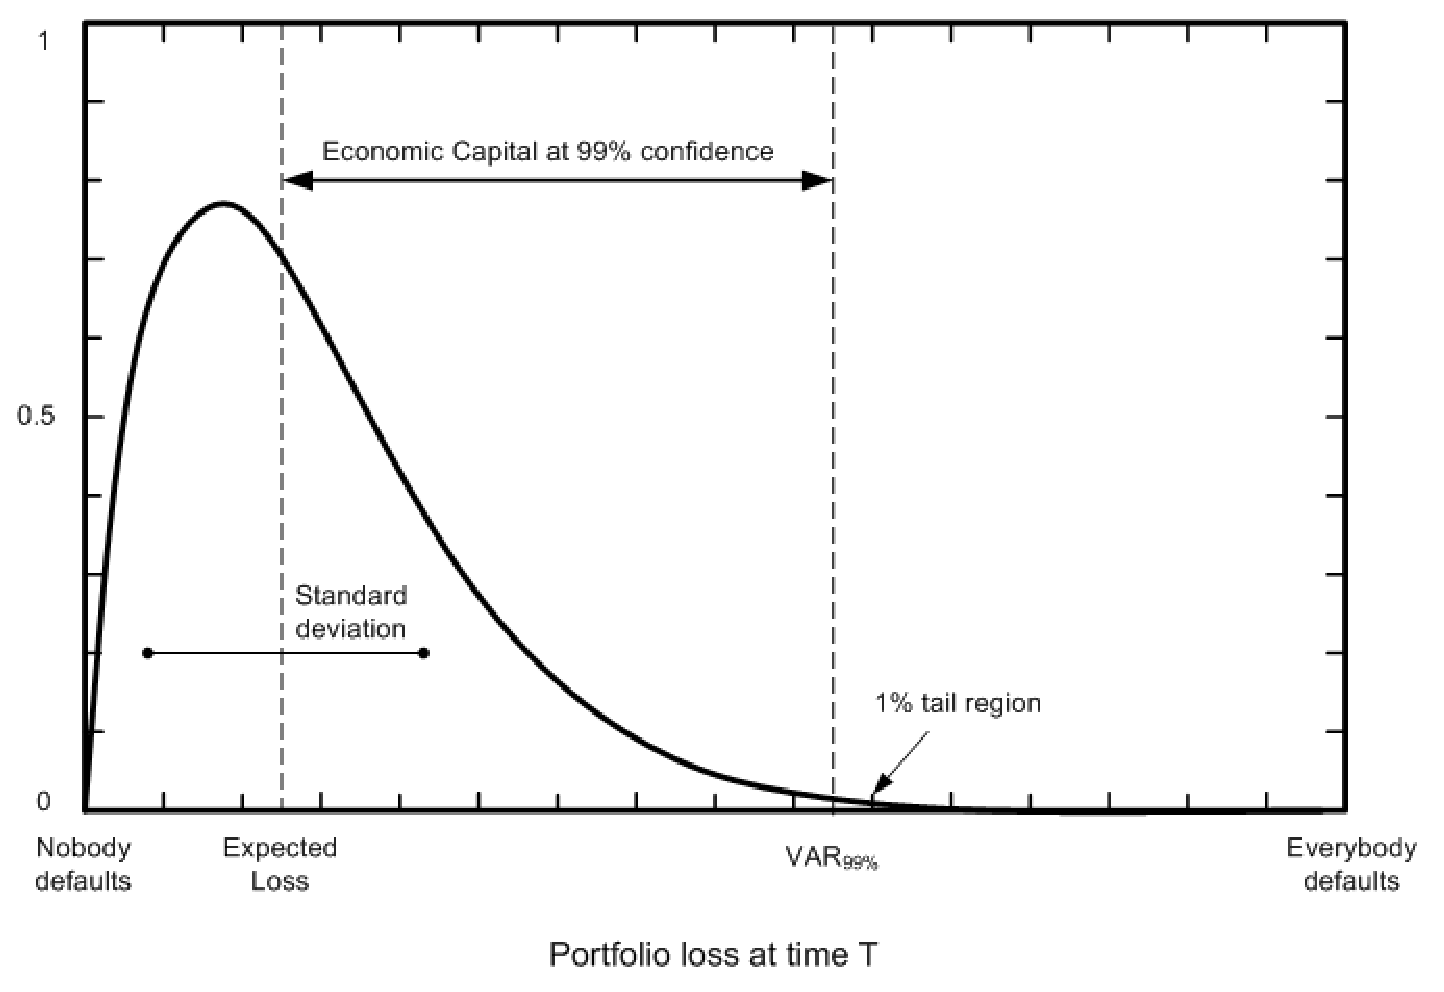
\includegraphics[height=7cm, angle=0]{./images/creditvar.eps}
\caption{Portfolio value at time $T$}
\label{creditvar}
\end{center}
\end{figure}

\paragraph{Ejemplo.} Calculemos el VAR de una cartera de cr\'editos
sencilla, de la que se puede obtener la distribuci\'on de las p\'erdidas de
forma expl\'icita. Sea una cartera de $1$ solo sector con $100$ clientes sin
correlaci\'on alguna entre ellos. Cada cliente tiene un activo que consiste en
devolver $1$ \euro al cabo de $T$ tiempo. Supongamos que el sistema de ratings
solamente contempla $2$ categor\'ias crediticias, no-Default y Default. La
probabilidad de hacer fallido al cabo de $T$ tiempo es $0.1$.
\newline
\newline
En este caso, se puede modelar la p\'erdida provocada por el impago del cliente
$i$ al cabo de $T$ tiempo como una variable aleatoria Bernouilli, $X_i \sim Ber(0.1)$.
La p\'erdida de la cartera al cabo de $T$ tiempo es la suma de las p\'erdidas de
cada cliente, $Z = \sum_{i=1}^{100} X_i$, que por definici\'on es una
variable aleatoria Binomial, $Z \sim B(100,0.1)$. El Teorema Central del
L\'imite nos permite aproximar $Z \sim B(100,0.1) \approx N(10, 9)$.
\newline
\newline
La p\'erdida esperada al cabo de $T$ tiempo es
\begin{displaymath}
\textrm{Expected Loss} = E(Z) \approx 10
\end{displaymath}

Calculemos el VAR al nivel de confianza $99\%$:
\begin{displaymath}
VAR_{99\%} = \textrm{inf}\{z | F_Z(z) \leq 99\%\}
\end{displaymath}
Teniendo en cuenta que $Z \approx N(10, 9)$, entonces
\begin{displaymath}
P(10 + \sqrt{9} \cdot X \leq VAR_{99\%}) = 99\%
\end{displaymath}
donde $X \sim N(0,1)$. Consultamos las tablas cdf de la Normal(0,1)
\begin{displaymath}
\frac{\textrm{VAR}_{99\%} - 10}{3} = 2.33
\end{displaymath}
Finalmente calculamos el $VAR_{99\%}$
\begin{displaymath}
\textrm{VAR}_{99\%} = 2.33 \cdot 3 + 10 = 16.99
\end{displaymath}

El Capital Econ\'omico al nivel de confianza $99\%$ es:
\begin{displaymath}
\textrm{Economic Capital}_{99\%}(Z) = \textrm{VAR}_{99\%}(Z) - E(Z) = 16.99 - 10 = 6.99
\end{displaymath}

Este ejemplo no es significativo debido a que se han realizado dos supuestos
que en el mundo real no se cumplen: todos los creditores se modelan de la misma 
forma y los fallidos son independientes. Se obtiene que la distribuci\'on de las 
p\'erdidas de la cartera a tiempo $T$ se aproxima a una variable aleatoria Normal,
cosa que no concuerda con las observaciones reales, que muestran que la
distribuci\'on de las p\'erdidas es fuertemente asim\'etrica respecto a la p\'erdida
esperada.



%***************************************************************************
%
% CreditCruncher - A portfolio credit risk valorator
% Copyright (C) 2004 Gerard Torrent
%
% This program is free software; you can redistribute it and/or
% modify it under the terms of the GNU General Public License
% as published by the Free Software Foundation; either version 2
% of the License.
%
% This program is distributed in the hope that it will be useful,
% but WITHOUT ANY WARRANTY; without even the implied warranty of
% MERCHANTABILITY or FITNESS FOR A PARTICULAR PURPOSE.  See the
% GNU General Public License for more details.
%
% You should have received a copy of the GNU General Public License
% along with this program; if not, write to the Free Software
% Foundation, Inc., 59 Temple Place - Suite 330, Boston, MA 02111-1307, USA.
%
%
% resolution.tex - TeX documentation file
% --------------------------------------------------------------------------
%
% 2005/01/22 - Gerard Torrent [gerard@fobos.generacio.com]
%   . initial release
%
%***************************************************************************

\chapter{Resoluci\'on del problema}
\label{sec:resolution}

En este cap\'itulo se introducen los elementos usados para la resoluci\'on y
se describen dos m\'etodos de resoluci\'on basados en simulaci\'on:
Time-To-Default y Rating-Path.

%---------------------------------------------------------------------------

\section{Notaci\'on}

\begin{tabular}{|p{2.5cm}|p{9cm}|}
\hline
\textbf{Concepto} & \textbf{Descripci\'on} \\
\hline
\hline
$x_i$ & Componente $i$-esimo de $x$ \\
\hline
$x^i$ & Realizaci\'on $i$-esima de la variable aleatoria $X$ \\
\hline
\hline
$ns$ & N\'umero de sectores de la cartera \\
\hline
$nr$ & N\'umero de ratings del sistema de calificaci\'on \\
\hline
$nc$ & N\'umero de clientes de la cartera \\
\hline
$na_i$ &  N\'umero de activos del cliente $i$. $i \in \{1,\cdots,nc\}$\\
\hline
\hline
$s_i$ & Sector $i$-esimo. $i \in \{1,\cdots,ns\}$ \\
\hline
$r_i$ & Rating $i$-esimo. $i \in \{1,\cdots,nr\}$. $r_{nr}=Default$. \\
\hline
$c_i$ & Cliente $i$-esimo. $i \in \{1,\cdots,nc\}$ \\
\hline
\hline
$S_{t_0}$ & Curva spot de tipos de inter\'es en $t_0$. $S_{t_0}(t_k)$ es el
tipo de inter\'es de la curva en tiempo $t_k$ siendo $t_0 \leq t_k$\\
\hline
$\Upsilon(t_0,t_k, S_{t_0})$ & Funci\'on de transporte de $t_0$ a $t_k$ usando 
la curva spot $S_{t_0}$ \\
\hline
\hline
$Survival(r_i,t)$ & Funci\'on de supervivencia. Probabilidad que un cliente con 
rating inicial $r_i$ no haya hecho fallido en tiempo $t$\\
\hline
$M_T$ & Matriz de transici\'on a $T$ tiempo. Tiene dimensi\'on $nr \times nr$\\
\hline
$\Gamma$ & Matriz de correlaci\'on entre sectores. Dimensi\'on $ns \times ns$\\
\hline
$\Theta$ & Matriz de correlaci\'on entre clientes. Dimensi\'on $nc \times nc$\\
\hline
\hline
$X_{i,j}(t)$ & Valor del $j$-esimo activo del cliente $i$ en tiempo $t$. 
$i \in \{1,\cdots,nc\}$, $j \in \{0,\cdots,na_i\}$ \\
\hline
$Y_i(t)$ & Valor de los activos del cliente $i$ en tiempo $t$. $i \in \{1,\cdots,nc\}$ \\
\hline
$Z(t)$ & Valor de la cartera en tiempo $t$\\
\hline
\end{tabular}

%---------------------------------------------------------------------------

\section{Variables aleatorias correlacionadas. C\'opulas.}

Se recomienda la lectura de las referencias \cite{copu:wang} y 
\cite{copu:pitfalls}. Se trata de art\'iculos donde se explica que es una 
c\'opula, sus propiedades, como simularlas, creencias erroneas, etc.

\paragraph{Definici\'on.} Llamamos \emph{c\'opula}\index{C\'opula} a la funci\'on
de distribuci\'on de una variable aleatoria $n$-dimensional tal que sus distribuciones
marginales \index{Distribuciones marginales} son variables aleatorias $U[0,1]$.
\begin{displaymath}
C(u_1, \cdots,u_n)=P(U_1 \leq u_1, \cdots, U_n \leq u_n) \qquad U_k \sim U[0,1]
\end{displaymath}

\begin{figure}[!hb]
\begin{minipage}[c]{0.5\columnwidth}%
  \centering
  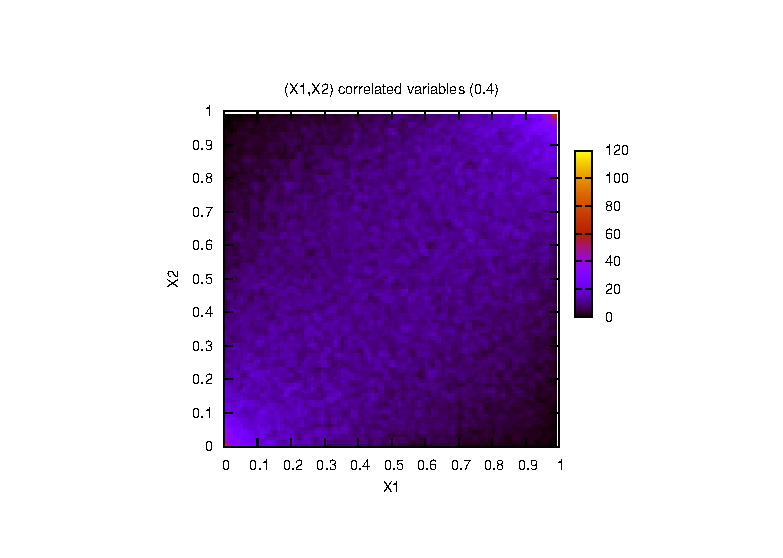
\includegraphics[height=5cm, angle=0]{./images/copula.eps}
\end{minipage}%
\hfill{}
\begin{minipage}[c]{0.5\columnwidth}%
  \centering
  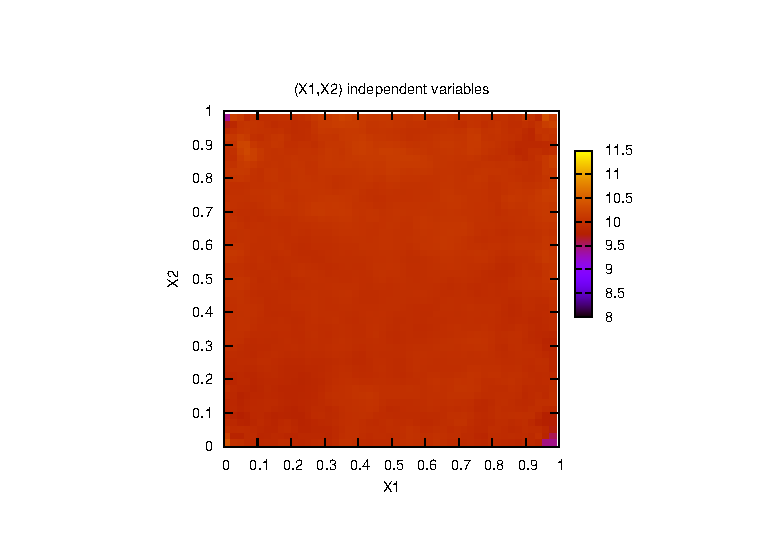
\includegraphics[height=5cm, angle=0]{./images/uniform.eps}
\end{minipage}%
\caption{Bivariate distribution plot with correlated and uncorrelated variables}
\label{copulas}
\end{figure}

\paragraph{Teorema.} \index{Teorema de Sklar} Toda variable aleatoria $n$-dimensional
puede separarse en las distribuciones seguidas por sus componentes (las distribuciones
marginales) y una c\'opula. Sea $F$ una funci\'on de distribuci\'on $n$-dimensional y
$f_1,\cdots, f_n$ sus marginales. El teorema de Sklar asegura que existe una 
c\'opula $C$ tq.
\begin{displaymath}
F(x_1, \cdots,x_n) = C(f_1(x_1), \cdots, f_n(x_n)) 
\end{displaymath}

\paragraph{Observaci\'on.} Una variable aleatoria $n$-dimensional no est\'a 
determinada por sus marginales y correlaciones entre estas. Dicho de otra
forma, existen infinitas formas de combinar las distribuciones marginales
 a trav\'es de c\'opulas de forma que cumplan las correlaciones. Las distribuciones 
el\'ipticas (que incluyen la distribuci\'on multinomial) son una excepci\'on. 

%---------------------------------------------------------------------------

\section{El m\'etodo de Monte Carlo}

Se recomienda la lectura de la referencia \cite{mc:mervyn}. Se trata de los 
apuntes para una clase del profesor Mervyn Marasinghe. Se expone el m\'etodo 
de Monte Carlo y las t\'ecnicas de reducci\'on de la varianza.

\paragraph{Definici\'on.} Dado un conjunto de observaciones, $x^1, \cdots, x^n$,
de la variable aleatoria $X$, definimos la \emph{funci\'on de distribuci\'on emp\'irica}
\index{Funci\'on de distribuci\'on emp\'irica} como:
\begin{displaymath}
\widetilde{F_X(k)} = \frac{1}{n} \sum_{i=1}^{n} I_{(-\infty,k]}(x^i) \qquad
I_{[-\infty,k]}(x) = \left\{
\begin{array}{ll}
1 & \textrm{ if } x \in (-\infty,k] \cr
0 & \textrm{ otherwise}
\end{array}
\right.
\end{displaymath}

\paragraph{Proposici\'on.} La funci\'on de distribuci\'on emp\'irica tiende a 
la funci\'on de distribuci\'on al incrementar el n\'umero de observaciones.
\begin{displaymath}
\qquad \lim_{n\to\infty} \widetilde{F_X} = F_X
\end{displaymath}

\paragraph{Definici\'on.} Sea $X$ una variable aleatoria con funci\'on de 
distribuci\'on conocida, $F$. El \emph{m\'etodo de Monte Carlo}\index{M\'etodo
de Monte Carlo} consiste en obtener la funci\'on de distribuci\'on empirica de
la variable aleatoria $H(X)$ usando el siguiente m\'etodo:
\begin{displaymath}
\begin{array}{ccc}
F_X                 &     \quad       & \widetilde{F_{H(X)}}    \cr
\downarrow          &     \quad       & \uparrow                \cr
\textrm{simulation} &     \quad       & \textrm{empirical } cdf \cr
\downarrow          &     \quad       & \uparrow                \cr
x^1,\cdots,x^n      & \longrightarrow & H(x^1),\cdots,H(x^n)
\end{array}
\end{displaymath}

\paragraph{Observaci\'on.} Problemas aparentemente no relacionados con las 
variables aleatorias pueden reformularse como un problema donde intervenga
una variable aleatoria y ser resueltos por el m\'etodo de Monte Carlo. El 
ejemplo cl\'asico es obtener el valor de la integral de la funci\'on $W$ entre 
$0$ y $1$. Lo reformulamos de la siguiente forma:
\begin{displaymath}
\int_{0}^{1} W(u) du = \int_{0}^{1} W(u) \phi(u) du = E[W(U)]
\end{displaymath}
donde $U \sim U[0,1]$ y $\phi(u) = \textrm{pdf}(U) = 1$. La \'ultima igualdad se
establece usando la preposici\'on enunciada en el ap\'endice \ref{apendix:stats}.
Finalmente la integral se aproxima calculando la media de un conjunto de puntos
con distribuci\'on $W(U)$.

%---------------------------------------------------------------------------

\section{Valor de un activo}

\paragraph{Definici\'on.} Definimos la funci\'on \emph{indicador del momento de 
fallido}\index{Indicador del momento de fallido} de la forma siguiente:
\begin{displaymath}
I(t) = \left\{
\begin{array}{ll}
1 & \textrm{ if client has defaulted at time } t \cr
0 & \textrm{ otherwise}
\end{array}
\right.
\end{displaymath}

\paragraph{Definici\'on.} Definimos la funci\'on \emph{indicador de actividad}
\index{Indicador de actividad} de la forma siguiente:
\begin{displaymath}
J(t) = \left\{
\begin{array}{ll}
0 & \textrm{ if client is defaulted at time } t\cr
1 & \textrm{ otherwise}
\end{array}
\right.
\end{displaymath}

\begin{figure}[!hb]
\begin{center}
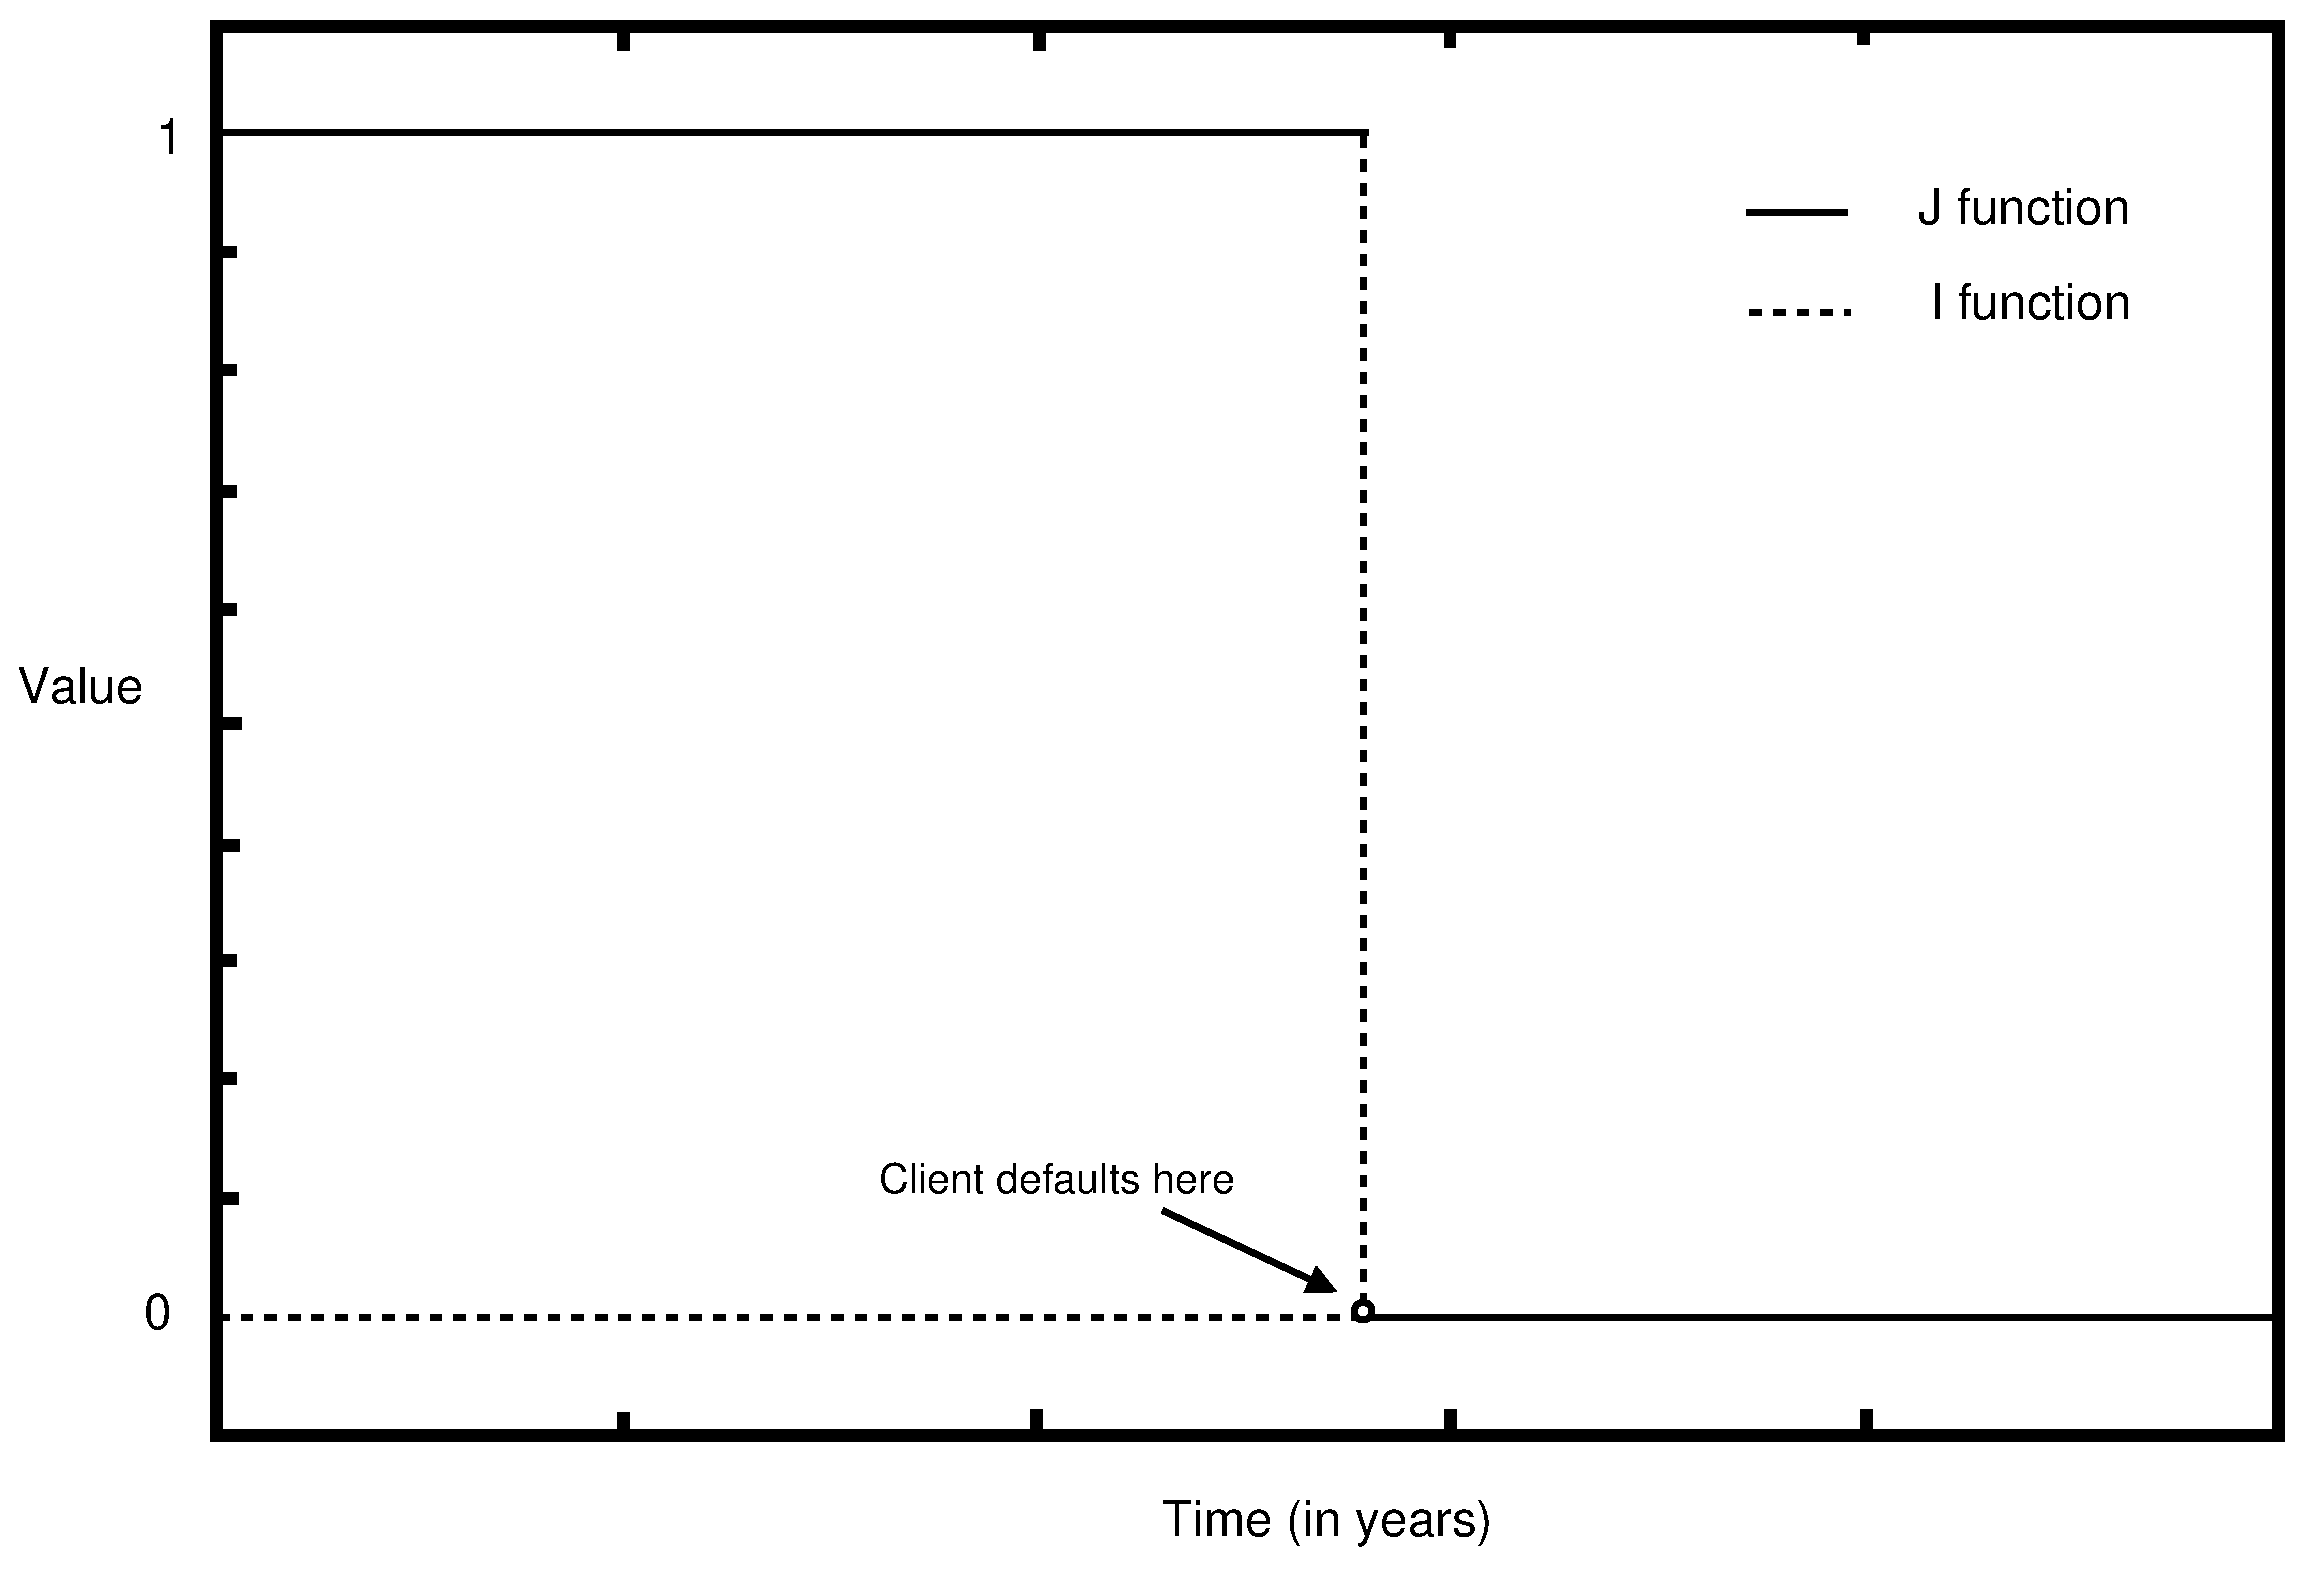
\includegraphics[width=10cm,angle=0]{./images/functionsIJ.eps}
\caption{Functions $I(t)$ and $J(t)$}
\label{functionsIJ}
\end{center}
\end{figure}

\paragraph{Proposici\'on.} Podemos expresar $J(t)$ en funci\'on de $I(t)$ de la
forma siguiente:
\begin{displaymath}
J(t) = \prod_{t_k=t_0}^{t} (1-I(t_k))
\end{displaymath}

\paragraph{Definici\'on.} Definimos el valor del activo $j$ del cliente $i$ en 
tiempo $t$ como:
\begin{displaymath}
\begin{array}{rl}
X_{i,j}(t) = \sum_{t_k=t_0}^{t} & \textrm{cashflow}(t_k) \cdot \Upsilon(t_k,t_0, S_{t_0}) \cdot J(t_k) \cr
                              + & \textrm{netting}(t_k)  \cdot \Upsilon(t_k,t_0, S_{t_0}) \cdot I(t_k)
\end{array}
\end{displaymath}

\paragraph{Observaci\'on.} Conocidas las caracter\'isticas de un activo y 
la curba spot, el valor de un activo en tiempo $t_k$ solamente depende de 
la funci\'on $I(t)$. Equivalentemente, solo depende del momento en que el
cliente hace fallido.


\section{Valor de la cartera}

\paragraph{Definici\'on.} Definimos el valor de la cartera en tiempo $t$ como:
\begin{displaymath}
Z(t) = \sum_{i=0}^{nc} Y_i(t) = \sum_{i=0}^{nc} \sum_{j=0}^{na_i} X_{i,j}(t)
\end{displaymath}

\paragraph{Observaci\'on.} El valor de la cartera solamente depende de 
$I_1(t), \cdots, I_{nc}(t)$, donde $I_i(t)$ es el indicador del momento 
de fallido en tiempo $t$ del cliente $i$. Equivalentemente, solo depende 
de los instantes en los que los clientes de la cartera hacen fallido.

\paragraph{Proposici\'on.} Construimos la funci\'on $H$ del m\'etodo de Monte 
Carlo de la forma siguiente:
\begin{displaymath}
H(I_1(t_0),\cdots,I_1(t_k),\cdots,I_{nc}(t_0),\cdots,I_{nc}(t_k)) = Z(T)
\end{displaymath}


\section{M\'etodo Time-To-Default}


El m\'etodo Time-To-Default consiste en simular el valor de la cartera a partir 
del la simulaci\'on del tiempo de fallido de cada uno de los clientes.

c\'opula -> funci\'on supervivencia -> valoraci\'on cartera

\begin{figure}[!hb]
\begin{center}
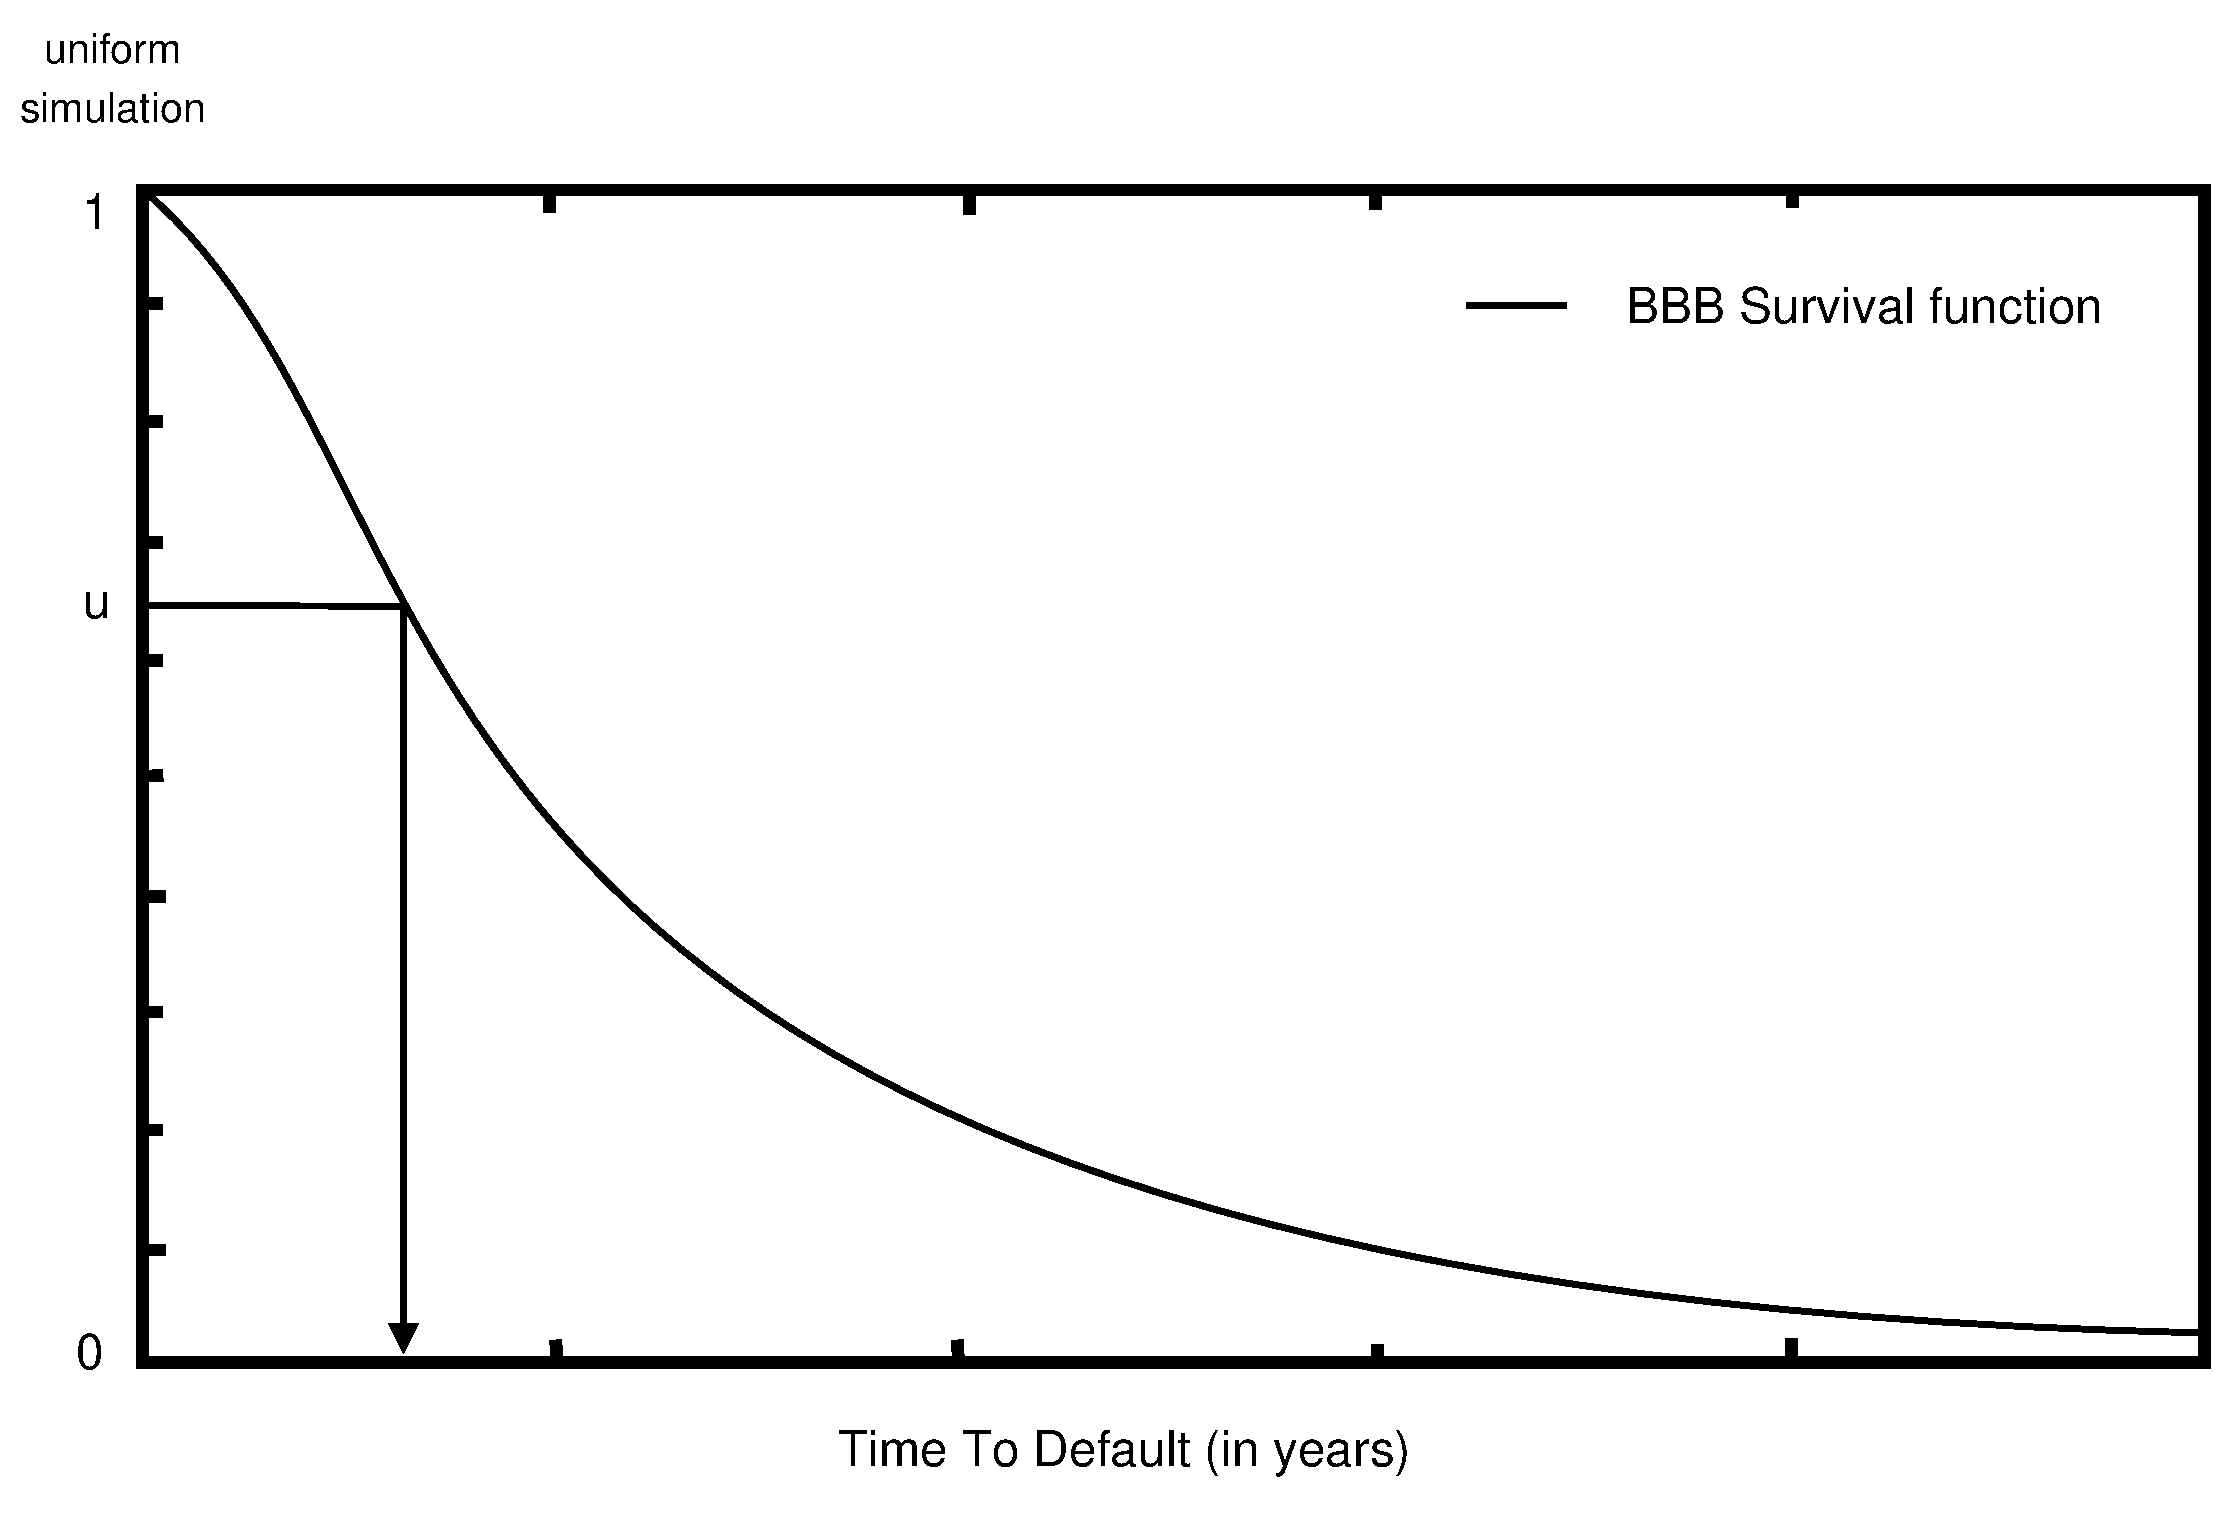
\includegraphics[width=10cm,angle=0]{./images/simttd.eps}
\caption{Simulaci\'on del tiempo hasta el fallido del rating $BBB$}
\label{simttd}
\end{center}
\end{figure}


\section{M\'etodo Rating-Path}
c\'opula -> matriz transici\'on -> valoraci\'on cartera

\begin{figure}[!hb]
\begin{center}
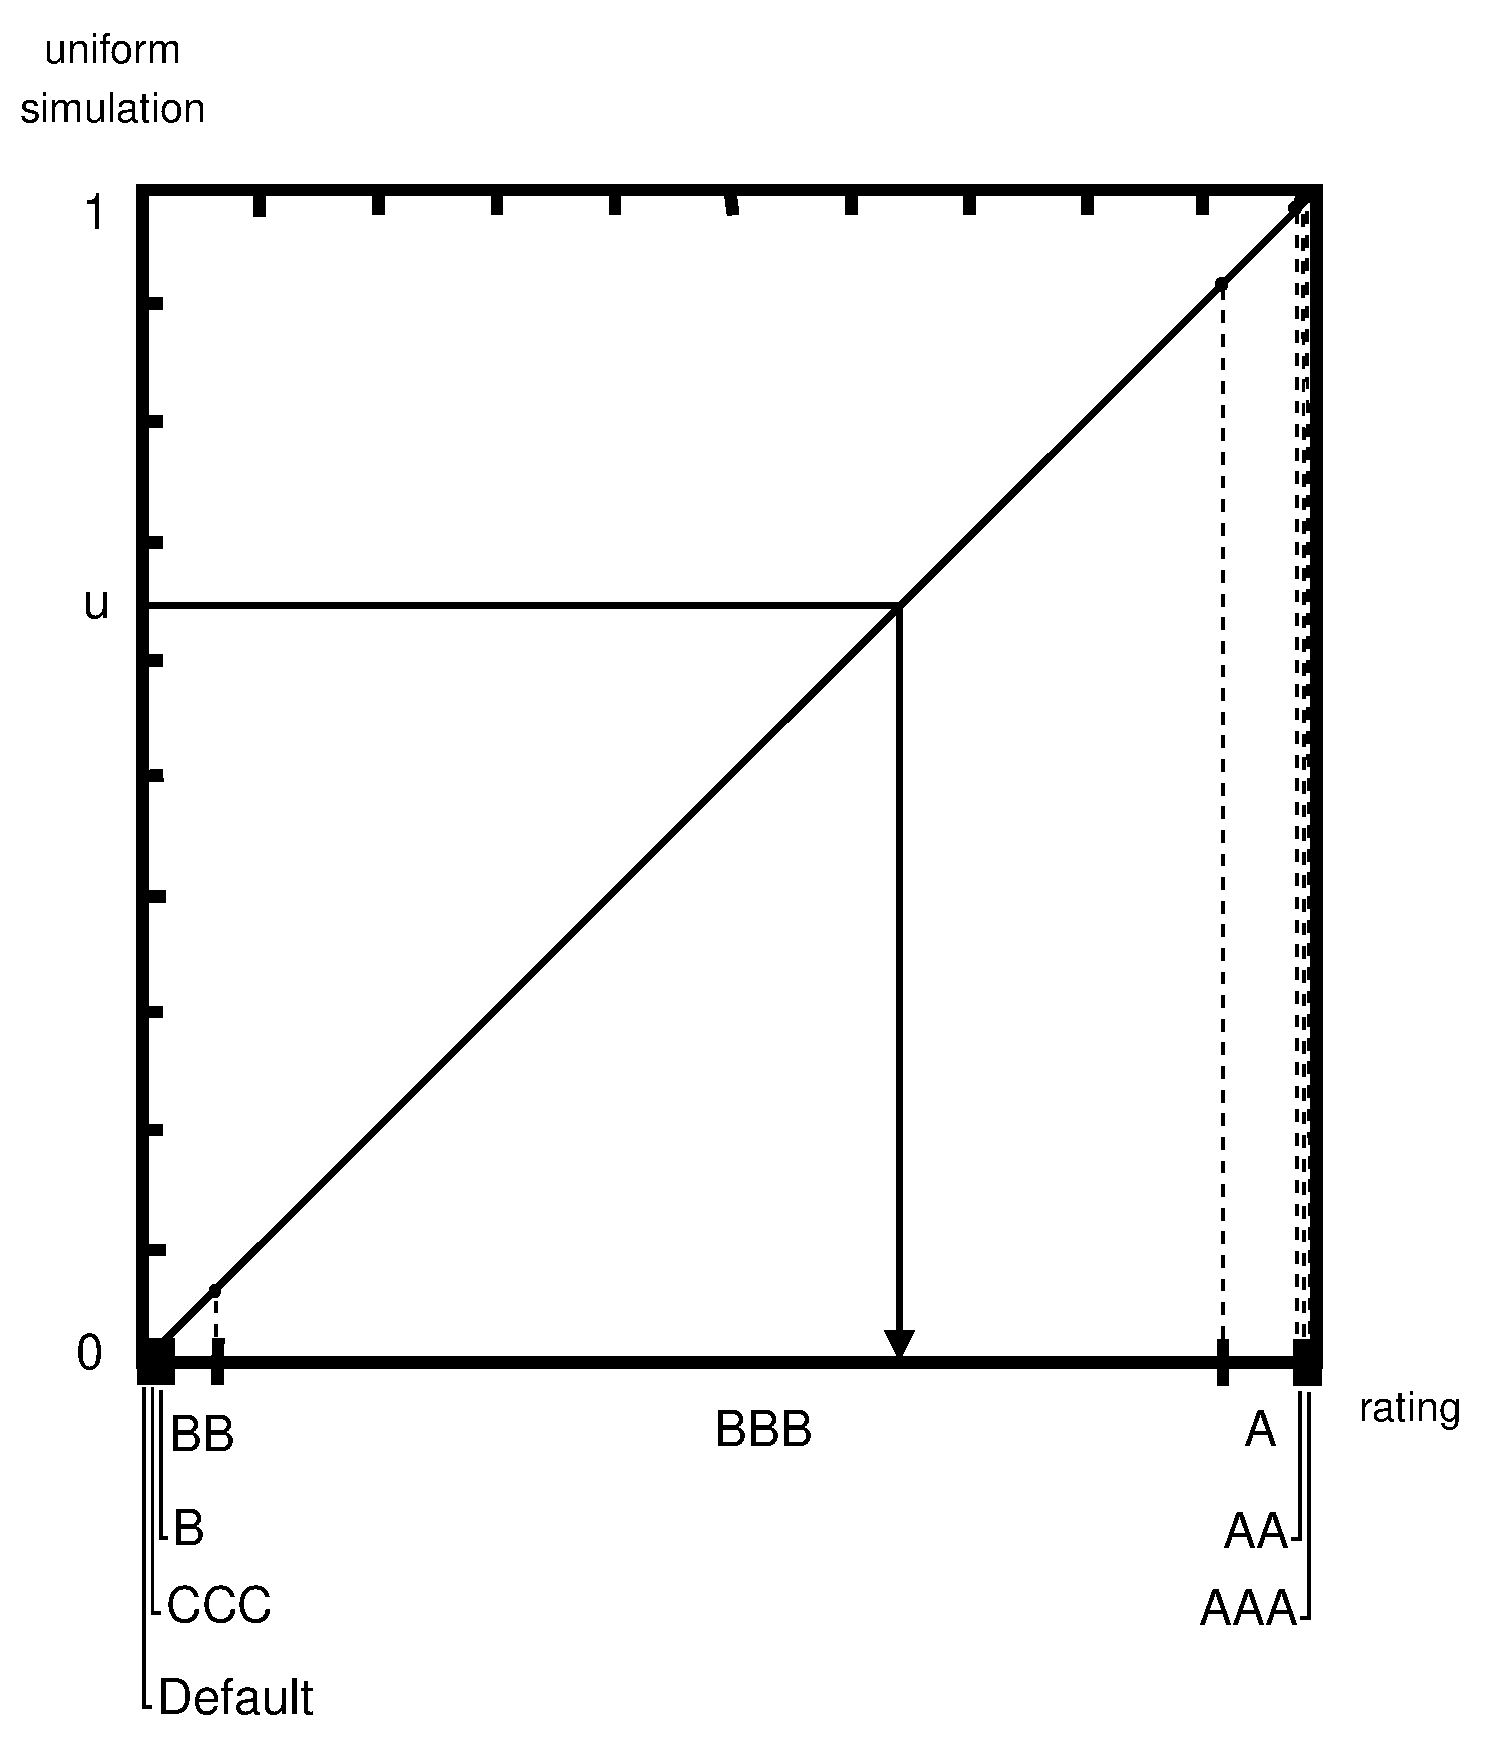
\includegraphics[width=7cm,angle=0]{./images/simrp.eps}
\caption{Simulaci\'on de la evoluci\'on del rating $BBB$ a $T$ tiempo}
\label{simrp}
\end{center}
\end{figure}


\subsection{Valoraci\'on de la cartera}
valoraci\'on activo -> valoraci\'on cliente -> valoraci\'on cartera

\subsection{Distribuci\'on del valor de la cartera}
calculo del valor esperado, calculo del VAR, etc.

%---------------------------------------------------------------------------

\section{Valoraci\'on del riesgo}

El m\'etodo de Monte Carlo genera $N$ realizaciones, $\{z_1,z_2,z_3,\cdots,z_N\}$,
de la variable aleatoria $Z$ (valor de la cartera) que permiten obtener la funci\'on
de distribuci\'on emp\'irica. A continuaci\'on se exponen los estimadores usados
y el $\alpha$-intervalo de confianza. CreditCruncher utiliza el entorno \emph{R}
\footnote{http://www.r-project.org} para realizar los c\'alculos estad'isticos.
Para mas informaci\'on acerca de \emph{R} v\'ease \cite{stats:R}.

\paragraph{Expected value.} F\'ormula extraida de \cite{stats:schaum} basada en el
teorema del l\'imite central.
\begin{displaymath}
\mu_Z = \widehat{\mu_Z} \pm \phi^{-1}\left(\frac{1-\alpha}{2}\right) \cdot \frac{\widehat{\sigma_Z}}{\sqrt{N}}
\end{displaymath}

\paragraph{Desviaci\'on est\'andar.} F\'ormula extraida de \cite{stats:schaum} basada en el
teorema del l\'imite central.
\begin{displaymath}
\sigma_Z = \widehat{\sigma_Z} \pm \phi^{-1}\left(\frac{1-\alpha}{2}\right) \cdot \frac{\widehat{\sigma_Z}}{\sqrt{2N}}
\end{displaymath}

\paragraph{VAR-Quantile.} Fijado un nivel de $VAR = 1-x$
\begin{displaymath}
q_{Z,x} = \widehat{q_{Z,x}} \pm \textrm{stderr}(q_{Z,x})
\end{displaymath}
Donde el error est\'andar del quantil, $\textrm{stderr}(q_{Z,x})$, lo calculamos usando
el m\'etodo de Maritz-Jarrett (basado en el estad\'istico de orden). F\'ormula extraida
de \cite{quant:algor}.


%***************************************************************************
%
% CreditCruncher - A portfolio credit risk valorator
% Copyright (C) 2004 Gerard Torrent
%
% This program is free software; you can redistribute it and/or
% modify it under the terms of the GNU General Public License
% as published by the Free Software Foundation; either version 2
% of the License.
%
% This program is distributed in the hope that it will be useful,
% but WITHOUT ANY WARRANTY; without even the implied warranty of
% MERCHANTABILITY or FITNESS FOR A PARTICULAR PURPOSE.  See the
% GNU General Public License for more details.
%
% You should have received a copy of the GNU General Public License
% along with this program; if not, write to the Free Software
% Foundation, Inc., 59 Temple Place - Suite 330, Boston, MA 02111-1307, USA.
%
%
% implementation.tex - TeX documentation file
% --------------------------------------------------------------------------
%
% 2005/01/22 - Gerard Torrent [gerard@fobos.generacio.com]
%   . initial release
%
%***************************************************************************

\chapter{Implementaci\'on de la soluci\'on}
\label{sec:implementation}

\section{Validaciones}

TODO: describir las validaciones realizadas


\begin{figure}[!hb]
\begin{center}
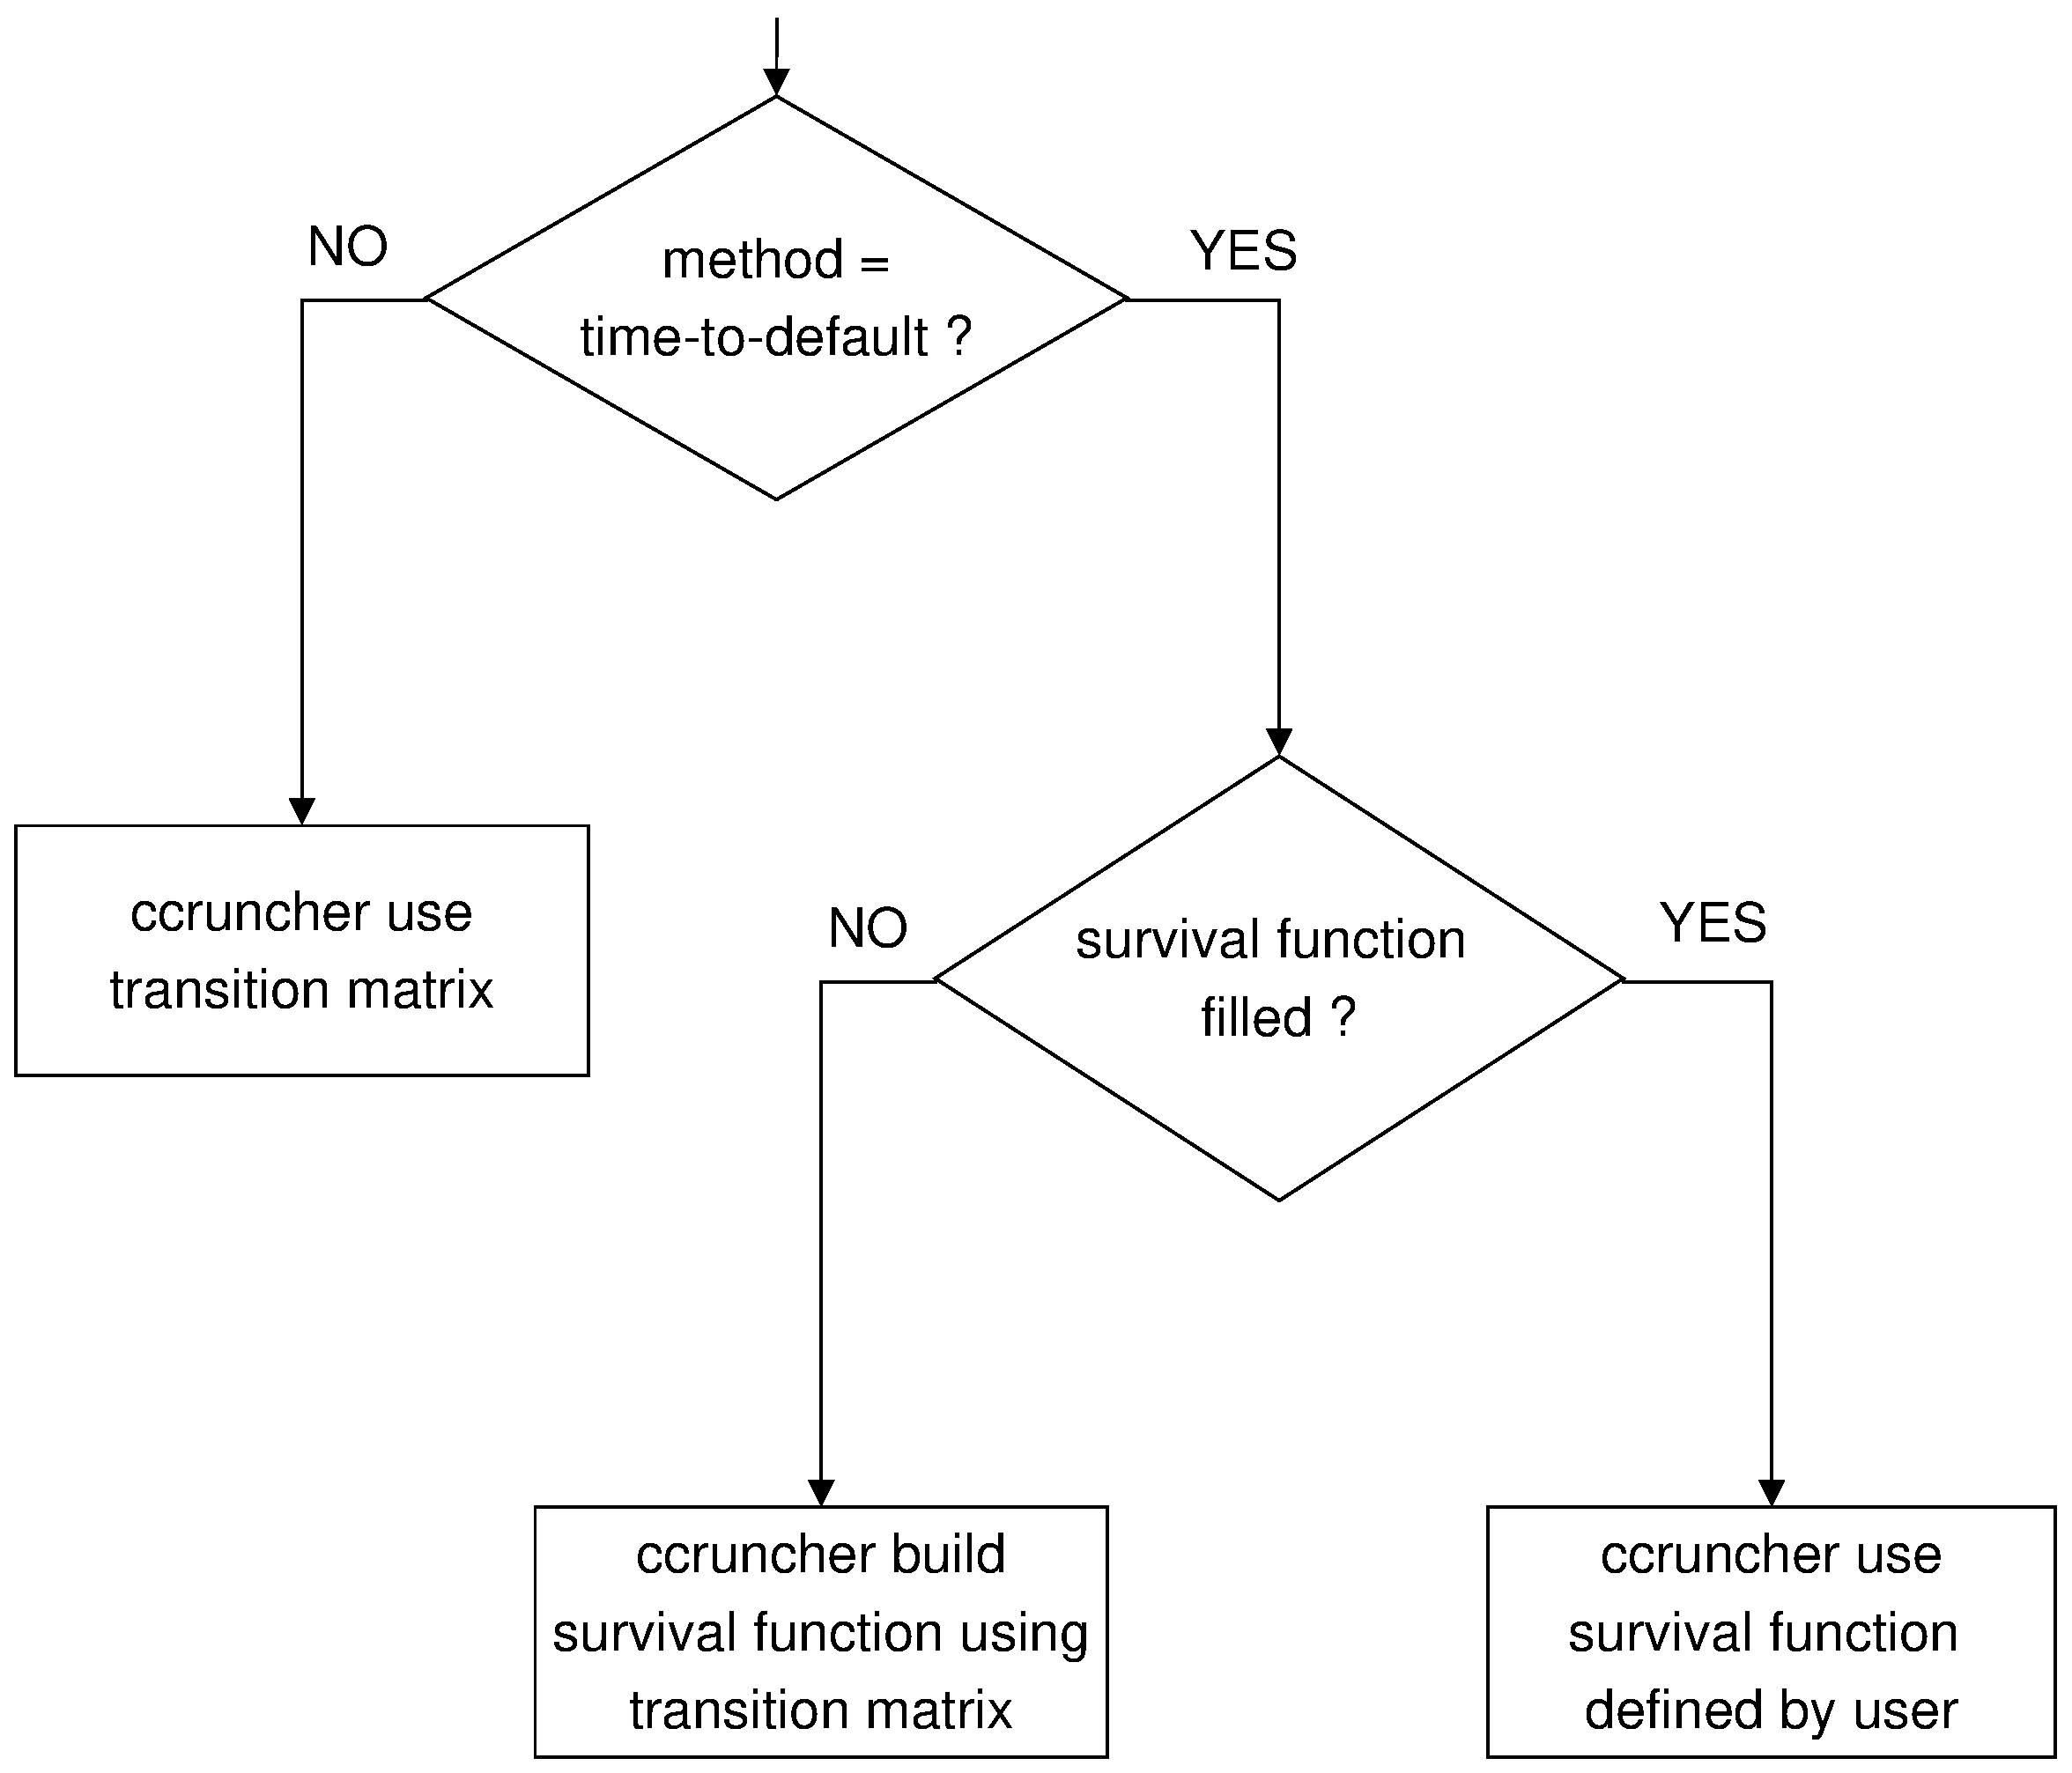
\includegraphics[width=10cm,angle=0]{./images/decisiontree1.eps}
\caption{Decisi\'on en funci\'on del m\'etodo}
\label{functionsIJ}
\end{center}
\end{figure}

precalculo de los valores en los nodos


\section{Proceso de agregaci\'on}

TODO: descripcion de los agregadores y metodo usado para evitar recalculo 
de los activos en cada simulacion + Agregaci\'on de productos


\section{Dimensiones del problema}

TODO: Estimaciones de uso de memoria, estimaci\'on del numero de operaciones,
estimacion del tiempo de computo


\section{Convergencia de la soluci\'on}

TODO: N\'umero de iteraciones necesarias, aceleraci\'on de la convergencia
usando metodolog\'ia antithetic

convergencia media, varianza, var (estimadores, graficos, etc.)

\appendix

%***************************************************************************
%
% CreditCruncher - A portfolio credit risk valorator
% Copyright (C) 2004 Gerard Torrent
%
% This program is free software; you can redistribute it and/or
% modify it under the terms of the GNU General Public License
% as published by the Free Software Foundation; either version 2
% of the License.
%
% This program is distributed in the hope that it will be useful,
% but WITHOUT ANY WARRANTY; without even the implied warranty of
% MERCHANTABILITY or FITNESS FOR A PARTICULAR PURPOSE.  See the
% GNU General Public License for more details.
%
% You should have received a copy of the GNU General Public License
% along with this program; if not, write to the Free Software
% Foundation, Inc., 59 Temple Place - Suite 330, Boston, MA 02111-1307, USA.
%
%
% appendices.tex - TeX documentation file
% --------------------------------------------------------------------------
%
% 2005/01/22 - Gerard Torrent [gerard@fobos.generacio.com]
%   . initial release
%
%***************************************************************************

\chapter{Ap\'endices}
\label{sec:apendixes}

%---------------------------------------------------------------------------
\section{Conceptos b\'asicos de estad\'istica}
\label{apendix:stats}

\paragraph{Definici\'on.} Llamamos funci\'on de distribuci\'on o cdf de la
variable aleatoria $X$ a la funci\'on $F$ que cumple:
\begin{displaymath}
F(x) = P(X \leq x)
\end{displaymath}

\paragraph{Definici\'on.} Llamamos funci\'on de probabilidad o densidad o pdf
 de la variable aleatoria $X$ a la funci\'on $f$ que cumple:
\begin{displaymath}
f(x) = \int_{-\infty}^{x} f(t) dt
\end{displaymath}

\paragraph{Proposici\'on.} Sea $X$ una variable aleatoria continua con
funci\'on de densidad $f_X(x)$. La funci\'on de densidad de $Y=H(X)$ siendo 
$H(.)$ mon\'otona (estrictamente creciente o estrictamente decreciente) es:
\begin{displaymath}
f_Y(y) = f_X(H^{-1}(y))\cdot \left| \frac{d(H^{-1}(y))}{dy} \right|
\end{displaymath}

\paragraph{Esperanza.} Definimos la esperanza de una variable aleatoria 
discreta de la forma siguiente:
\begin{displaymath}
E(X) = \sum_{i} i \cdot P(X=i)
\end{displaymath}
En el caso de una variable aleatoria continua con funci\'on de distribuci\'on 
$f(x)$ la esperanza se expresa como:
\begin{displaymath}
E(X) = \int_{-\infty}^{\infty} x \cdot f(x) dx
\end{displaymath}

\paragraph{Varianza.} Definimos la varianza de una variable aleatoria discreta 
de la forma siguiente:
\begin{displaymath}
Var(X) = \sum_{i} (i-E(X))^2 \cdot P(X=i)
\end{displaymath}
En el caso de una variable aleatoria continua con funci\'on de distribuci\'on 
$f(x)$ la varianza se expresa como:
\begin{displaymath}
Var(X) = \int_{-\infty}^{\infty} (x-E(X))^2 \cdot f(x) dx
\end{displaymath}

\paragraph{Covarianza.} Definimos la covarianza entre dos variables 
aleatorias $X$ e $Y$ de la forma siguiente:
\begin{displaymath}
Cov(X,Y) = E(X \cdot Y) - E(X) \cdot E(Y)
\end{displaymath}

\paragraph{Correlaci\'on.} Definimos la correlaci\'on, $\rho$, entre dos 
variables aleatorias $X$ e $Y$ de la forma siguiente:
\begin{displaymath}
\rho_{X,Y} = \frac{Cov(X,Y)}{\sqrt{Var(x) \cdot Var(Y)}}
\end{displaymath}

\paragraph{Proposici\'on.} Sea $X$ una variable aleatoria continua con
funci\'on de densidad $f(x)$ y $H(x)$ una funci\'on diferenciable. Entonces:
\begin{displaymath}
E(H(X)) = \int_{-\infty}^{\infty} H(x) \cdot f(x) dx
\end{displaymath}


%---------------------------------------------------------------------------

\section{La variable aleatoria de Bernoulli}

\paragraph{Definici\'on.} La variable aleatoria discreta Bernouilli, $X$, se 
utiliza para modelar fen\'omenos que solamente pueden tomar dos estados, 
$0$ y $1$, con probabilidades $p$ y $(1-p)$ respectivamente. La notaremos 
como $X \sim Ber(p)$:
\begin{displaymath}
P(X=0) = (1 - p) \qquad   P(X=1) = p \qquad p \in [0,1]
\end{displaymath}
 
\paragraph{Esperanza.} La esperanza de una variable aleatoria Bernouilli $X \sim Ber(p)$ 
es $p$. Este resultado es la aplicaci\'on directa de la definici\'on de esperanza 
para una variable aleatoria discreta:
\begin{displaymath}
E(X) = \sum_{i} i \cdot P(X=i) = 1 \cdot p + 0 \cdot (1-p) = p
\end{displaymath}

\paragraph{Varianza.} La varianza de una variable aleatoria Bernouilli $X \sim Ber(p)$ 
es $p \cdot (1-p)$. Este resultado es la aplicaci\'on directa de la definici\'on 
de varianza para una variable aleatoria discreta:
\begin{displaymath}
Var(X)= \sum_{i} (i-E(X))^2 \cdot P(X=i) = (1-p)^2 \cdot p + (-p)^2 \cdot (1-p) = p \cdot (1-p)
\end{displaymath}
 
\paragraph{Simulaci\'on.} La simulaci\'on de una variable Bernouilli 
$X \sim Ber(p)$ la realizamos de la siguiente forma:
\begin{displaymath}
x= \left\{
\begin{array}{cc}
0 & u \in [0,1-p) \cr
1 & u \in [1-p,1]
\end{array}
\right.
\qquad u \sim U[0,1]
\end{displaymath}

%---------------------------------------------------------------------------

\section{La variable aleatoria Binomial}

\paragraph{Definici\'on.} La suma de $n$ variables aleatorias Bernoulli, $Ber(p)$,  
independientes e id\'enticamente distribuidas es una variable aleatoria discreta, 
$X$ que llamamos Binomial, $X \sim B(n,p)$.
\begin{displaymath}
P(X=k) = {n \choose k} \cdot p^k \cdot (1-p)^{n-k} \qquad {n \choose k} = \frac{n!}{k! \cdot (n-k)!}
\qquad k \in \{0, \cdots, n\}
\end{displaymath}

\paragraph{Esperanza.} La esperanza de una variable aleatoria Binomial 
$X \sim B(n,p)$ es:
\begin{displaymath}
E(X) = n \cdot p
\end{displaymath}

\paragraph{Varianza.} La varianza de una variable aleatoria Binomial 
$X \sim B(n,p)$ es:
\begin{displaymath}
Var(X)= n \cdot p \cdot (1-p)
\end{displaymath}

\paragraph{Proposici\'on.} El Teorema Central del L\'imite nos permite, en el
caso de $n$ grandes, aproximar la distribuci\'on discreta Binomial por una 
distribuci\'on continua Normal:
\begin{displaymath}
B(n,p) \approx N\left(n p, n p (1-p)\right)
\end{displaymath}


%---------------------------------------------------------------------------

\section{La variable aleatoria Normal}

\paragraph{Definici\'on.} Decimos que una variable aleatoria continua $Z$ es 
una Normal con media $\mu$ y desviaci\'on est\'andar $\sigma$, 
$Z \sim N(\mu, \sigma^2)$ si tiene la siguiente funci\'on de densidad:
\begin{displaymath}
f(x) = \frac{1}{\sigma \sqrt{2 \pi}} e^{-\frac{(x-\mu)^2}{2 \sigma^2}}
\end{displaymath}

\paragraph{Esperanza.} La esperanza de una variable aleatoria Normal 
$X \sim N(\mu,\sigma^2)$ es:
\begin{displaymath}
E(X) = \mu
\end{displaymath}

\paragraph{Varianza.} La varianza de una variable aleatoria Normal 
$X \sim N(\mu,\sigma^2)$ es:
\begin{displaymath}
Var(X)= \sigma^2
\end{displaymath}

\paragraph{Simulaci\'on.} Para la generaci\'on de una realizaci\'on, $z$, de 
una variable aleatoria normal $Z \sim N(\mu, \sigma^2)$ utilizamos el siguiente 
algoritmo:
\begin{displaymath}
z = \mu + \sigma\cdot \sqrt{-2 ln(u_1)} \cdot cos(2 \pi \cdot u_2)
\qquad u_1, u_2 \sim U[0,1]
\end{displaymath}

\paragraph{Definici\'on.} Decimos que una variable aleatoria continua 
$n$-dimensional, $Z$, es una Normal con media $\vec{\mu}$ y matriz de 
covarianza $\Sigma$, $Z \sim N(\vec{\mu}, \Sigma)$, si tiene la 
siguiente funci\'on de densidad:
\begin{displaymath}
f(\vec{x}) = \frac{1}{\sqrt{(2 \pi)^n \left| \Sigma \right|}} 
exp\left\{-\frac{1}{2}\left(\vec{x}-\vec{\mu})^{\top} \Sigma^{-1} (\vec{x}-\vec{\mu}) \right)\right\}
\end{displaymath}
donde $\left|\Sigma\right|$ es el determinante de la matriz de covarianzas 
$\Sigma$, y $\Sigma^{-1}$ es la inversa de la matriz $\Sigma$.

\paragraph{Simulaci\'on.} Para la generaci\'on de una realizaci\'on, $\vec{z}$, 
de una variable aleatoria normal $Z \sim N(\vec{\mu}, \Sigma)$ utilizamos el 
siguiente algoritmo:
\begin{displaymath}
\vec{z} = \vec{\mu} + \Sigma^{1/2} \vec{x}
\qquad x_i \sim N[0,1]
\end{displaymath}
La matriz $\Sigma^{1/2}$ la calculamos usando el algoritmo de Cholesky. Sabemos 
que existe soluci\'on debido a que $\Sigma$ es definida positiva por tratarse
de una matriz de covarianzas.

%---------------------------------------------------------------------------

\section{C\'alculo de la raiz de una matriz}

\paragraph{Definici\'on.}
Diremos que 2 matrices $A$ y $B$ de orden $n$ son semejantes si existe una 
matriz, $P$, de orden $n$ con $det(P) \neq 0$ tal que 
$B = P^{-1} \cdot A \cdot P$.


\paragraph{Proposici\'on.} Si dos matrices $A$ y $B$ son semejantes 
($B = P^{-1} \cdot A \cdot P$) entonces:
\begin{displaymath}
det(A) = det(B)
\end{displaymath}
\begin{displaymath}
B^n = P^{-1} \cdot A^{n} \cdot P
\end{displaymath}

\paragraph{Definici\'on.} 
Diremos que una matriz $A$ de orden $n$ es diagonalizable si es semejante a una 
matriz diagonal $D$, o sea, $A = P^{-1} \cdot D \cdot P$ siendo $det(D) \neq 0$.

\paragraph{Proposici\'on.} 
Para que una matriz $A$ sea diagonalizable es necesario y suficiente que:
\begin{itemize}
\item Los valores propios de $A$ sean todos reales
\item Los $n$ vectores propios de $A$ sean independientes
\end{itemize}

\paragraph{Proposici\'on.}
Si una matriz $A$ es diagonalizable ($A = P^{-1} \cdot D \cdot P$) entonces: 
\begin{itemize}
\item $D$ es una matriz diagonal compuesta por los valores propios de la matriz $A$
\item $P$ es la matriz formada por los vectores propios de la matriz $A$
\end{itemize}

\paragraph{Resultado.}
Sea $A$ la ra\'iz $n$-esima de una matriz diagonalizable $B$. Entonces:
\begin{displaymath}
A^n = B = P^{-1} \cdot D \cdot P 
\Longrightarrow  
A = \sqrt[n]{B} = P^{-1} \cdot \sqrt[n]{D} \cdot P
\end{displaymath} 

%---------------------------------------------------------------------------

\section{Algoritmo de la c\'opula normal}

Sea $\Sigma_1$ la matriz de correlaci\'on a cumplir por la c\'opula. Observemos 
que se trata tambi\'en de la matriz de covarianzas al valer $1$ los elementos
de la diagonal.
\begin{displaymath}
\Sigma_1 = \left( 
\begin{array}{cccc}
1          & \rho_{12} & \ldots & \rho_{1n} \cr
\rho_{21} & 1          & \ldots & \rho_{2n} \cr
\vdots    & \vdots    & \ddots & \vdots   \cr
\rho_{n1} & \rho_{n2} & \ldots & 1
\end{array}
\right)
\end{displaymath}

\paragraph{Paso 1.} Creamos la matrix de covarianzas $\Sigma_2$ transformando 
la matriz $\Sigma_1$ componente a componente:
\begin{displaymath}
\Sigma_2 = \left( 
\begin{array}{cccc}
2 sin(\frac{\pi}{6})           & 2 sin(\rho_{12} \frac{\pi}{6}) & \ldots & 2 sin(\rho_{1n} \frac{\pi}{6})\cr
2 sin(\rho_{21} \frac{\pi}{6}) & 2 sin(\frac{\pi}{6})           & \ldots & 2 sin(\rho_{2n} \frac{\pi}{6})\cr
\vdots                          & \vdots                          & \ddots  & \vdots   \cr
2 sin(\rho_{n1} \frac{\pi}{6}) & 2 sin(\rho_{n2} \frac{\pi}{6}) & \ldots & 2 sin(\frac{\pi}{6})
\end{array}
\right)
\end{displaymath}

\paragraph{Paso 2.} A la matriz $\Sigma_2$ le aplicamos el algoritmo de 
Cholesky para obtener la matrix triangular inferior $B$ cumpliendo 
$\Sigma_2 = B \cdot B^{\top}$:
\begin{displaymath}
B = 
\left(
\begin{array}{cccc}
b_{11}   & 0        & \ldots & 0       \cr
b_{21}   & b_{22}   & \ldots & 0       \cr
\vdots  & \vdots  & \ddots & \vdots \cr
b_{n1}   & b_{n2}   & \ldots & b_{nn}
\end{array}
\right)
\end{displaymath}

\paragraph{Paso 3.} Simulamos $n$ variables aleatorias $N(0,1)$ independientes:
\begin{displaymath}
\vec{Y}^{\top}=(Y_1, \cdots, Y_n)^{\top} \qquad Y_k \sim N(0,1) \textrm{ independientes}
\end{displaymath}

\paragraph{Paso 4.} Simulamos una variable n-dimensional $Z \sim N(\vec{0}, \Sigma_2)$
haciendo:
\begin{displaymath}
\vec{Z}^{\top} = 
\left(
\begin{array}{c}
Z_1 \cr
\vdots \cr
Z_n
\end{array}
\right) 
=
\left(
\begin{array}{cccc}
b_{11}   & 0        & \ldots & 0       \cr
b_{21}   & b_{22}   & \ldots & 0       \cr
\vdots  & \vdots  & \ddots & \vdots \cr
b_{n1}   & b_{n2}   & \ldots & b_{nn}
\end{array}
\right)
\left(
\begin{array}{c}
Y_1 \cr
\vdots \cr
Y_n
\end{array}
\right) 
 = B \cdot \vec{Y}^{\top}
\end{displaymath}

\paragraph{Paso 5.} Finalmente obtenemos la simulaci\'on de la c\'opula, $\vec{X}$.
\begin{displaymath}
\vec{X}^{\top} = (X_1, \cdots, X_n)^{\top} = (\Phi(Z_1), \cdots, \Phi(Z_n))^{\top}
\end{displaymath}
donde $\Phi(x)$ es la funci\'on de distribuci\'on de la Normal est\'andar
\begin{displaymath}
\Phi(x) = \int_{-\infty}^{x} \frac{1}{\sqrt{2 \pi}} e^{-\frac{t^2}{2}} dt
\end{displaymath}



\bibliography{refs}
\bibliographystyle{plain}

\printindex

\end{document}
